\documentclass[journal]{IEEEtran}

\usepackage{graphicx}
\usepackage{amsmath}
\usepackage{amssymb}
\usepackage{booktabs}
\usepackage{url}
\usepackage{multirow}
\usepackage{array}
\usepackage[hidelinks]{hyperref}

% --- diagram support: the schematic figures are drawn in TikZ ---------------
\usepackage{tikz}
\usetikzlibrary{arrows.meta,positioning,calc,fit,backgrounds,shapes.geometric}

\definecolor{bblue}{HTML}{2A78D6}
\definecolor{borange}{HTML}{EB6834}
\definecolor{btint}{HTML}{DCE9F8}
\definecolor{bwarm}{HTML}{FDECE4}
\definecolor{bink}{HTML}{0B0B0B}
\definecolor{binkb}{HTML}{52514E}
\definecolor{bpaper}{HTML}{F4F4F2}
\definecolor{bline}{HTML}{C8C7C2}

\tikzset{
  icon/.style={line width=0.5pt, draw=#1, line cap=round, line join=round},
  pics/ic person/.style n args={1}{code={\begin{scope}[icon=#1]
      \draw (0,0.085) circle (0.055);
      \draw (-0.095,-0.095) .. controls (-0.095,0.02) and (0.095,0.02) .. (0.095,-0.095);
    \end{scope}}},
  pics/ic funnel/.style n args={1}{code={\begin{scope}[icon=#1]
      \draw (-0.125,0.10) -- (0.125,0.10) -- (0.033,-0.02) -- (0.033,-0.11)
            -- (-0.033,-0.07) -- (-0.033,-0.02) -- cycle;
    \end{scope}}},
  pics/ic store/.style n args={1}{code={\begin{scope}[icon=#1]
      \draw (-0.09,0.085) -- (-0.09,-0.085) arc (180:360:0.09 and 0.042) -- (0.09,0.085);
      \draw (0,0.085) ellipse (0.09 and 0.042);
      \draw (-0.09,0.0) arc (180:360:0.09 and 0.042);
    \end{scope}}},
  pics/ic scale/.style n args={1}{code={\begin{scope}[icon=#1]
      \draw (0,-0.115) -- (0,0.105);
      \draw (-0.135,0.07) -- (0.135,0.07);
      \draw (-0.135,0.07) -- (-0.19,-0.025) -- (-0.08,-0.025) -- cycle;
      \draw (0.135,0.07) -- (0.08,-0.025) -- (0.19,-0.025) -- cycle;
      \draw (-0.07,-0.115) -- (0.07,-0.115);
    \end{scope}}},
  pics/ic check/.style n args={1}{code={\begin{scope}[icon=#1,line width=0.8pt]
      \draw (-0.11,0.0) -- (-0.03,-0.08) -- (0.12,0.09);
    \end{scope}}},
  pics/ic half/.style n args={1}{code={\begin{scope}[icon=#1]
      \draw (0,0) circle (0.10);
      \fill[#1] (0,0) -- (0.10,0) arc (0:180:0.10) -- cycle;
    \end{scope}}},
  pics/ic warn/.style n args={1}{code={\begin{scope}[icon=#1]
      \draw[rounded corners=0.6pt] (0,0.12) -- (0.13,-0.10) -- (-0.13,-0.10) -- cycle;
      \draw (0,0.05) -- (0,-0.02);
      \fill[#1] (0,-0.058) circle (0.013);
    \end{scope}}},
  pics/ic link/.style n args={1}{code={\begin{scope}[icon=#1]
      \draw[rounded corners=1.1pt] (-0.14,-0.042) rectangle (0.012,0.052);
      \draw[rounded corners=1.1pt] (-0.012,-0.052) rectangle (0.14,0.042);
    \end{scope}}},
  pics/ic doc/.style n args={1}{code={\begin{scope}[icon=#1]
      \draw (-0.08,-0.11) -- (-0.08,0.11) -- (0.03,0.11) -- (0.08,0.058)
            -- (0.08,-0.11) -- cycle;
      \draw (0.03,0.11) -- (0.03,0.058) -- (0.08,0.058);
      \draw (-0.045,0.018) -- (0.045,0.018);
      \draw (-0.045,-0.04) -- (0.045,-0.04);
    \end{scope}}},
  pics/ic probe/.style n args={1}{code={\begin{scope}[icon=#1]
      \draw (-0.02,0.028) circle (0.072);
      \draw (0.032,-0.024) -- (0.11,-0.10);
    \end{scope}}},
  pics/ic tree/.style n args={1}{code={\begin{scope}[icon=#1]
      \draw (0,0.085) -- (0,0.02); \draw (-0.115,0.02) -- (0.115,0.02);
      \draw (-0.115,0.02) -- (-0.115,-0.035); \draw (0.115,0.02) -- (0.115,-0.035);
      \fill[#1] (0,0.115) circle (0.030);
      \fill[#1] (-0.115,-0.065) circle (0.030);
      \fill[#1] (0.115,-0.065) circle (0.030);
    \end{scope}}},
  pics/ic shield/.style n args={1}{code={\begin{scope}[icon=#1]
      \draw (0,0.115) -- (0.10,0.07) -- (0.10,-0.03)
            .. controls (0.10,-0.085) and (0.05,-0.10) .. (0,-0.125)
            .. controls (-0.05,-0.10) and (-0.10,-0.085) .. (-0.10,-0.03)
            -- (-0.10,0.07) -- cycle;
    \end{scope}}},
}

\newcommand{\ico}[2]{\tikz[baseline=-0.62ex]{\pic{ic #1={#2}};}}

\tikzset{
  bx/.style={draw=bink, fill=white, rounded corners=1.6pt, line width=0.45pt,
             align=center, font=\scriptsize, inner sep=2.8pt,
             execute at begin node={\hyphenpenalty=10000\exhyphenpenalty=10000}},
  bxhi/.style={bx, draw=bblue, fill=btint, line width=0.75pt},
  bxwarn/.style={bx, draw=borange, fill=bwarm, line width=0.75pt},
  bxsoft/.style={bx, fill=bpaper, draw=binkb, line width=0.4pt},
  flow/.style={-{Latex[length=3.6pt,width=2.8pt]}, draw=bink, line width=0.5pt},
  faint/.style={-{Latex[length=3pt,width=2.4pt]}, draw=binkb, line width=0.35pt},
  escal/.style={-{Latex[length=3.2pt,width=2.6pt]}, draw=borange, line width=0.5pt,
              dash pattern=on 1.7pt off 1.3pt},
  band/.style={rounded corners=2.5pt, draw=bline, line width=0.5pt, fill=white},
  bandlab/.style={font=\scriptsize\itshape, text=binkb, inner sep=1.5pt},
  capt/.style={font=\scriptsize\itshape, text=binkb, align=center},
}

\begin{document}
\raggedbottom

\title{When Departments Disagree: A Blockchain Reconciled Agentic AI Framework for Institutional Knowledge and Employee Guidance}

\author{Khaled Almi'ani, Nedal Ababneh and Nur Siyam%
\thanks{K. Almi'ani is with the Faculty of Computer Information Science, Higher Colleges of Technology, P.O. Box 1626, Fujairah, United Arab Emirates (corresponding author, e-mail: kalmiani@hct.ac.ae).}%
\thanks{N. Ababneh is with the Information Security Engineering Department, Abu Dhabi Polytechnic, Abu Dhabi, United Arab Emirates.}%
\thanks{N. Siyam is with the Faculty of Computer Information Science, Higher Colleges of Technology, Sharjah, United Arab Emirates.}}

\maketitle

\begin{abstract}
Organisations hold one body of procedural knowledge per department, each under its own policy regime. However, employee questions routinely cross departmental boundaries. Guidance that answers them must therefore be assembled from departments that were never obliged to agree. Accordingly, this paper presents BRAIN, a Blockchain Reconciled Agentic Institutional Network. Each department operates an agentic assistant over its own blockchain anchored partition. An authority lattice on a permissioned ledger declares which department is authoritative for each claim type. A deterministic protocol then reconciles the departmental drafts into one attributable answer or an explicit escalation. Evaluation used a generated five year corpus of 1082 artefacts, 400 scenarios and a simulated agent. Baselines matched on retrieval affordances attain either coverage or refusal but never both. None exceeds 0.651 attribution, whereas the proposed framework reaches 0.870 coverage at 0.100 confident error with complete attribution. Six unfavourable findings are reported in full. The setting is shared services in a government entity, where mandate is allocated in writing and revised through dated circulars. A registration mapping onto instruments such an entity already holds is stated, together with a four phase deployment path and the conditions each phase must demonstrate.
\end{abstract}

\begin{IEEEkeywords}
Agentic artificial intelligence, blockchain, multi-agent systems, organisational knowledge management, retrieval augmented generation, knowledge conflict, provenance, audit, human oversight, escalation, permissioned ledgers.
\end{IEEEkeywords}

\section{Introduction}

\IEEEPARstart{O}{rganisational} knowledge is not held in one place. Distinct bodies of procedure are maintained by finance and by legal. Human resources, information security and operations each maintain their own. Every department interprets the same events through a different mandate, and every department is authoritative over a different part of what the organisation must decide. This separation is not a defect to be engineered away, since it is how organisations manage specialisation. Along these lines, the boundaries between such groups have been characterised as pragmatic rather than merely informational, because knowledge at a boundary is invested in a local practice and must be transformed rather than simply transferred in order to cross it \cite{carlile2004transforming}. Additionally, the routines through which departmental work is actually performed have been argued to diverge from the routines as written \cite{feldman2003routines}. The documents that describe a department are therefore an incomplete account of its practice.

The difficulty appears when a question crosses those boundaries. For instance, a case officer onboarding an overseas supplier that will process customer records is not asking a procurement question and then a contracting question. That officer is not asking an information security question and a service continuity question in sequence either. The officer is asking one question whose correct answer is assembled from four departments that have never been required to agree with one another, that may be working from different circular versions, and that may attach different meanings to the same classification term. Coordination of this kind has been studied as an organisational problem in its own right, as the management of dependencies among activities \cite{malone1994coordination}, and knowledge sharing between units of a single firm has been shown to occur under simultaneously cooperative and competitive conditions \cite{tsai2002coopetition}. The employee, however, receives none of that context. The employee receives one answer from the organisation.

Generative assistants grounded in an organisation's own material do not resolve this difficulty and can obscure it. Retrieval augmented generation produces more specific and more factual output than a purely parametric model \cite{huang2026ragsurvey}, which is why such assistants are increasingly placed in front of staff. The standard deployment pools every departmental document into a single index. However, once the departmental provenance of a passage is flattened into one corpus, a contradiction between two departments becomes indistinguishable from redundancy between two copies of the same rule. The generator then selects whichever formulation the retriever ranked first. The measurements reported in Section~IV quantify this behaviour. A pooled arrangement that retains department labels attributes 0.454 of its obligations correctly and issues 0.546 of them in the name of a department that does not own the matter. Such an arrangement answers confidently on an unsettled matter in 0.853 of the cases that require escalation. A pooled arrangement additionally equipped with a currency filter and an exact existence lookup recovers much of the lost coverage, at 0.706. That arrangement still issues 0.349 of its obligations in the name of a department that does not own the matter. The deficiency is therefore one of mandate rather than one of retrieval. Notably, these outcomes are consistent with the wider literature. Knowledge conflict between retrieved passages has been categorised as a distinct failure mode \cite{xu2024conflicts}. Generated citations have been shown to frequently fail to support the statements they are attached to \cite{gao2023citations}. Models have also been shown to degrade on facts that have recently changed \cite{vu2024freshllms}.

Providing each department with its own assistant restores provenance and surfaces the disagreement, yet it leaves the employee holding several answers and no principled way to combine them. Multi-agent architectures built on large language models have advanced quickly, including agents that debate from assigned stances under a judge \cite{liang2024debate} and agent societies that reproduce believable social behaviour \cite{park2023generative}, and the collaboration mechanisms available to such agents have been studied as a design space \cite{zhang2024collaboration}. However, the dominant resolution mechanism in that literature is persuasion, in which agents exchange arguments until they converge or a referee model selects a winner. Persuasion is not the appropriate mechanism for an organisation, since whether the security department or the operations department prevails on a question of remote access is a matter of which department holds the mandate rather than of which agent argues more convincingly. Furthermore, a referee model is itself a source of bias, as strong model judges have been shown to be sensitive to the order in which candidates are presented \cite{wang2024unfair}. The measurements in Section~IV support this position. A referee over departmental drafts improves attribution only from 0.425 to 0.481. The silent wrong answer rate, which is confident assertion on a matter the organisation has not settled, remains at 0.884.

Two further properties are absent from both arrangements. The first property is accountability after the fact. An organisation whose composite advice proves incorrect must establish which department's rule was applied and what that department was shown at the time. The organisation must also establish whether the mandate under which the rule prevailed was the mandate in force on that date. Neither a pooled index nor a conversational agent ensemble retains such a record in a form that survives a later dispute, because both can be edited afterwards and neither commits the context that was served before the answer was produced. The second property is principled refusal, since an organisation frequently should not receive an answer at all. When two departments hold incompatible mandates over the same matter, or when the department that owns a mandatory part of the question has no rule in force, the appropriate output is an escalation naming the departments concerned. Systems that always answer convert an organisational disagreement into a confident sentence, whereas the capacity of a model to recognise what it does not know has been measured directly and found limited \cite{yin2023knowunknown,kamath2020selective}.

To address such a challenge, this paper combines a permissioned ledger with mandate aware generative agents. The proposed framework is named BRAIN, for Blockchain Reconciled Agentic Institutional Network. Figure~\ref{fig:framework} illustrates the conceptual workflow of the proposed framework across a departmental boundary. The framework consists of five components. The partition and the lattice come first, and the drafting, reconciliation and settlement components follow. The partition component holds each department's artefacts, signs them, binds them to the policy version under which they were issued and anchors them in Merkle batches. The lattice component declares which department owns each class of claim. The same component declares which departments are consulted on it and how precedence runs when owners disagree. The drafting component produces claims drawn from a closed vocabulary rather than prose. Every claim carries a modality, a condition and a policy version, together with citations to the anchored artefacts that were served. The reconciliation component detects conflicts among the departmental claim sets, classifies them into six mechanically distinguishable classes, and applies a fixed order of resolution rules whose outcome is either an attributable answer or an explicit escalation. The settlement component binds each outcome to the evidence that produced it and records it on the ledger.

\begin{figure*}[!t]
\centering
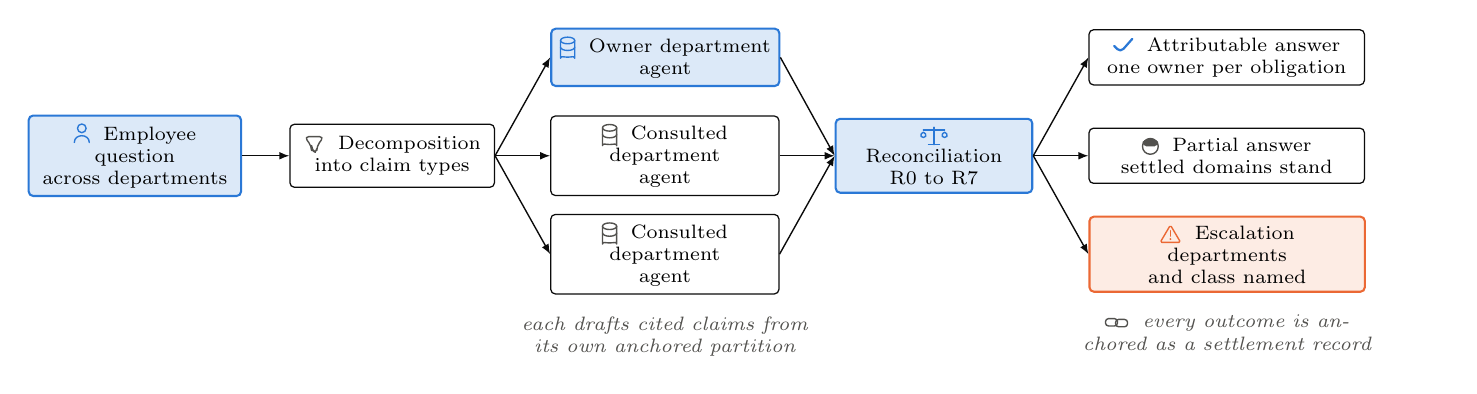
\begin{tikzpicture}
  \node[bxhi, text width=25mm, minimum height=8mm] (q)
    {\ico{person}{bblue}\; Employee question\\ across departments};
  \node[bx, right=6mm of q, text width=24mm, minimum height=8mm] (dec)
    {\ico{funnel}{binkb}\; Decomposition\\ into claim types};

  \node[bxhi, right=7mm of dec, text width=27mm, minimum height=7mm, yshift=12.5mm] (own)
    {\ico{store}{bblue}\; Owner department\\ agent};
  \node[bx, right=7mm of dec, text width=27mm, minimum height=7mm] (c1)
    {\ico{store}{binkb}\; Consulted department\\ agent};
  \node[bx, right=7mm of dec, text width=27mm, minimum height=7mm, yshift=-12.5mm] (c2)
    {\ico{store}{binkb}\; Consulted department\\ agent};

  \node[bxhi, right=7mm of c1, text width=23mm, minimum height=8mm] (rec)
    {\ico{scale}{bblue}\; Reconciliation\\ R0 to R7};

  \node[bx, right=7mm of rec, text width=33mm, minimum height=7mm, yshift=12.5mm] (o1)
    {\ico{check}{bblue}\; Attributable answer\\ one owner per obligation};
  \node[bx, right=7mm of rec, text width=33mm, minimum height=7mm] (o2)
    {\ico{half}{binkb}\; Partial answer\\ settled domains stand};
  \node[bxwarn, right=7mm of rec, text width=33mm, minimum height=7mm, yshift=-12.5mm] (o3)
    {\ico{warn}{borange}\; Escalation\\ departments and class named};

  \draw[flow] (q) -- (dec);
  \foreach \t in {own,c1,c2} \draw[flow] (dec.east) -- (\t.west);
  \foreach \s in {own,c1,c2} \draw[flow] (\s.east) -- (rec.west);
  \foreach \t in {o1,o2,o3} \draw[flow] (rec.east) -- (\t.west);

  \node[capt, below=1.6mm of c2, text width=40mm]
    {each drafts cited claims from its own anchored partition};

  \node[capt, below=1.6mm of o3, text width=54mm]
    {\ico{link}{binkb}\; every outcome is anchored as a settlement record};
\end{tikzpicture}
\caption{Conceptual workflow of the proposed framework across a departmental boundary.}
\label{fig:framework}
\end{figure*}

The setting in which this difficulty is sharpest is the one in which authority is allocated formally rather than negotiated. A government entity distributes mandate by law and by executive resolution, and also by a delegation of authority matrix and published terms of reference. Policies are revised through dated circulars rather than through silent edits. The question of which unit is authoritative over a class of decision therefore carries a written and versioned answer that predates any system built above it. Such an allocation is precisely the object that the authority lattice encodes. Accordingly, the proposed framework does not ask an entity to invent a governance structure but rather to declare in machine readable form the one under which it already operates, and thereafter to hold its automated guidance to it. Notably, the same entities are measured on the guidance they give to staff and to customers. An assistant that answers confidently where the entity has not decided therefore imposes a cost that its own service standards already recognise. Notably, agentic arrangements permit a model to act rather than merely to answer. Such arrangements raise that requirement rather than relax it. Accordingly, the mandate is treated here as a first class registered object and refusal as a first class outcome, whereas Section~VI relates both to the governance principles under which such a system would be deployed.

This work is organised around four research questions. RQ1 asks how frequently cross departmental guidance conflicts in a corpus with realistic version skew, how those conflicts distribute across the six proposed classes, and what proportion of them a pooled retrieval baseline is capable of surfacing at all. RQ2 asks whether departmental partitioning under a registered authority lattice improves the correctness and the attributability of composite guidance relative to pooled retrieval, to the concatenation of departmental answers and to a referee model. The second question also asks what that improvement costs. RQ3 asks whether escalation is well calibrated, which is to say whether the proposed framework refuses when the organisation genuinely holds no reconciled position and answers when it does. RQ4 asks how the proposed framework behaves when a departmental agent is captured and when a partition is poisoned. The same question covers fabricated citations, the exploitation of a superseded policy version and a compromised lattice registry.

The contributions of this work are summarised as follows. First, a departmental partition and a two stage anchoring scheme are defined. The issuing department, the policy version and the attested quality of every artefact are committed rather than inferred. A departmental root that is not covered by the cross department commitment for its epoch is inadmissible as evidence. Second, an authority lattice is specified as a versioned on chain artefact that maps claim types to owning and consulted departments together with a per subject precedence order, and the acyclicity condition that makes deterministic resolution possible is stated and checked at registration. Third, a taxonomy of six classes of cross departmental conflict is proposed with detection procedures over closed vocabulary claims. Two of those classes are jurisdiction overreach and silent omission, neither of which a pooled index can represent. Fourth, a reconciliation protocol is specified as an ordered rule set containing a completeness probe and terminating in an escalation state. A settlement registry is implemented in Solidity (0.8.20) that binds each answer to the served context, the claim set and the rule trace, together with the lattice version. Fifth, a reproducible evaluation is reported over eight experiments against six baselines together with two further arms matched to the proposed framework on retrieval affordances and on the capacity to refuse, with a language model in the loop employed only to fix the operating point rather than to score the output. Finally, six unfavourable findings are reported in full. The first three are a retrieval loss attributable to partitioning, a contradiction detection precision of 0.470 and a definitional detection recall of 0.590. The remaining three are a residual silent wrong answer rate of 0.100, a governance single point of failure that the measurements confirm and a pronounced sensitivity to modality drift, which is the one agent failure mode the operating point does not bound.

The remainder of this paper is organised as follows. Section~II surveys the related literature in three groups and states the gap that remains. Section~III describes the proposed framework and its five components. Section~IV reports the experimental configuration and the measured results of the eight experiments. Section~V addresses the four standard categories of validity threat. Section~VI relates the design to the governance principles under which such a system would be deployed and states what remains before it could be. Finally, Section~VII concludes the paper and outlines the intended future work.


\section{Related Work}

The literature relevant to the proposed framework is surveyed in three groups. Organisational knowledge boundaries supply the motivation. Agents and retrieval augmented generation supply the drafting and delivery mechanisms together with their documented failures. Blockchain provenance and conflict resolution supply the trust substrate, the settlement machinery and the measurement discipline.

\subsection{Organisational Knowledge Boundaries and Coordination}

Carlile \cite{carlile2004transforming} proposed a three level framework in which syntactic, semantic and pragmatic knowledge boundaries are matched to transfer, translation and transformation. That distinction maps onto three of the conflict classes proposed in Section~III. Along these lines, Feldman and Pentland \cite{feldman2003routines} distinguished the ostensive from the performative aspect of an organisational routine, which implies that a departmental record is an incomplete account of departmental practice. Malone and Crowston \cite{malone1994coordination} characterised coordination as the management of dependencies among activities, whereas Tsai \cite{tsai2002coopetition} reported that knowledge sharing between units of a single firm occurs under simultaneously cooperative and competitive conditions. In the context of delivering such knowledge to staff, Weber et al. \cite{weber2001lessons} surveyed deployed lessons learned systems and reported that stand alone repositories are under used unless the lesson is delivered inside the decision process that needs it. However, none of this literature addresses what a machine should do when two departments issue incompatible instructions to the same employee.

\subsection{Agents, Generative Collaboration and Retrieval Augmented Generation}

Wooldridge and Jennings \cite{wooldridge1995agents} consolidated the agent abstraction and its theoretical and practical treatments. Classical coordination protocols assume agents that pursue a shared goal, and a departmental agent is not such a member, since it is the delegate of a unit with its own mandate and its disagreement with another unit is legitimate rather than a coordination failure to be repaired. The literature that addresses precisely that case is the normative one. Jones and Sergot \cite{jones1996power} formalised institutionalised power, under which an act performed by the holder of a designated role counts as creating an institutional fact whereas the same act performed by any other agent does not, and Esteva et al. \cite{esteva2001institutions} specified electronic institutions in which such an allocation of roles and powers is enforced by the infrastructure rather than left to the agents. Along these lines, policy based management classified the modality conflicts that arise when several managers hold authority over overlapping targets and resolved them by registered precedence \cite{lupu1999conflicts}. In essence, this literature already holds that authority is a registered fact rather than an outcome of argument. The proposed framework inherits that position directly, since jurisdiction projection is a counts as condition and precedence is a registered priority among authorities. What the present setting adds is that the assertions being governed are drafted by generative agents whose output is untrusted. The institution must therefore bind every assertion to evidence committed before it was drafted.

More recently, agent societies built on large language models have been shown to reproduce believable individual and emergent social behaviour \cite{park2023generative}, and several proposals have examined how such agents should resolve disagreement. For instance, Liang et al. \cite{liang2024debate} encouraged divergent thinking by assigning opposing stances together with a judge, whereas Zhang et al. \cite{zhang2024collaboration} studied collaboration mechanisms as a design space. However, two properties of debate as a resolution mechanism are relevant here, namely that it settles by persuasion and that its arbiter is a model. Wang et al. \cite{wang2024unfair} demonstrated that strong model evaluators are sensitive to the presentation order of candidates and are therefore not neutral arbiters. An organisational mandate is not a preference to be judged but a registered fact about which department is entitled to decide, and the proposed framework accordingly replaces the model arbiter with that registered fact wherever the registry speaks.

Huang and Huang \cite{huang2026ragsurvey} surveyed retrieval augmented text generation and reported that grounding a generator in retrieved material improves factuality relative to a purely parametric model, which is the reason such assistants are increasingly placed in front of staff. For the retrieval stage itself, Robertson and Zaragoza \cite{robertson2009bm25} gave the reference treatment of the lexical relevance framework employed in this work. The failure modes are equally well documented. Ji et al. \cite{ji2023hallucination} surveyed hallucination together with its sources and mitigations. Gao et al. \cite{gao2023citations} demonstrated that models frequently emit citations that do not support their own statements. Xu et al. \cite{xu2024conflicts} categorised knowledge conflict between retrieved context and model parameters and among retrieved passages. Vu et al. \cite{vu2024freshllms} reported degradation on facts that have recently changed. Additionally, the corpus is an attack surface. Zhong et al. \cite{zhong2023poisoning} showed for dense retrievers that a small number of injected adversarial passages surface for a large fraction of unrelated queries. Greshake et al. \cite{greshake2023injection} showed that retrieved content can carry instructions that hijack the surrounding application. Notably, the capacity to decline is treated as a separate matter, where Kamath et al. \cite{kamath2020selective} traded coverage against accuracy through an explicit abstention threshold and Yin et al. \cite{yin2023knowunknown} measured the extent to which models recognise unanswerable questions and found it limited. In essence, the conflicts studied in this literature are conflicts of fact. The conflicts addressed in the present work are conflicts of mandate, which cannot be resolved by determining which passage is true.

\subsection{Blockchain Provenance, Conflict Resolution and Evaluation}

The canonical tamper evident construction is the hash tree, which yields inclusion proofs logarithmic in the number of leaves \cite{merkle1988signature}. Androulaki et al. \cite{androulaki2018fabric} described the execute, order and validate architecture of a modular permissioned ledger with pluggable consensus and identity. That description includes the channel mechanism that partitions state among subsets of participants. Castro and Liskov \cite{castro2002pbft} supplied the Byzantine fault model with proactive recovery under which such a ledger tolerates compromised participants. W\"{u}st and Gervais \cite{wust2018blockchain} gave the criteria under which a ledger is warranted at all, namely several writers that do not trust one another together with the absence of an operator all of them trust, and Eberhardt and Tai \cite{eberhardt2017offchain} systematised off-chaining as a family of patterns in which only commitments are written on chain. Sandhu et al. \cite{sandhu1996rbac} supplied the remaining primitive, namely role based models that express permissions as a mapping from roles to operations. The authority lattice proposed in this work is related to that mapping and differs from it in an important respect. Role based access control governs which department may read or write, whereas the lattice governs whose assertion prevails when two authorised departments assert incompatible obligations. That question is addressed by policy based management through precedence \cite{lupu1999conflicts}, and the present work carries the treatment over to generated rather than authored assertions. The public sector application of these primitives has been examined directly. Almi'ani et al. \cite{almiani2026government} surveyed the adoption of blockchain in government and reported transparency and trust as the recurring motivations. Al Suwaidi et al. \cite{almiani2024housing} proposed a ledger based framework for housing establishment support services, whereas Al-Jaziri et al. \cite{almiani2026skillchain} combined credential validation on a ledger with artificial intelligence for talent mapping in Dubai Government. Along these lines, the monitoring of decentralised applications has been expressed as deterministic finite automata over contract events \cite{almiani2024qos}. The trustworthiness of the inputs such systems consume has been addressed by graph based profiling of oracles \cite{almiani2023oracles} and by adaptive trust decay \cite{almiani2026trustdecay}. These proposals govern transactions and credentials rather than the assertions of departmental agents, which is the gap the present work addresses.

Konieczny and Pino P\'erez \cite{konieczny2002merging} supplied the logical treatment of merging several sources under integrity constraints together with the postulates a rational merging operator should satisfy, whereas Dong et al. \cite{dong2009conflicting} demonstrated that source dependence matters when resolving conflicting values, since a false value can spread through copying. However, these formalisms resolve conflicts by reference to consistency or to source reliability, neither of which is the operative criterion when two reliable departments hold incompatible mandates. Finally, the measurement apparatus employed in Section~IV is conventional, comprising discounted cumulated gain \cite{jarvelin2002ndcg} together with the randomisation and bootstrap significance procedures recommended by Smucker et al. \cite{smucker2007significance}.

Overall, the surveyed literature has not brought these groups together. The organisational literature establishes that departmental boundaries are pragmatic and that crossing them requires transformation, whereas it offers no machine representation of which boundary is authoritative for which decision. Normative multi-agent systems and policy based management establish that authority is a registered fact and supply the counts as condition and the precedence rule that the proposed framework adopts, whereas they govern assertions that are authored rather than generated and therefore need not bind an assertion to the evidence available when it was made. Their generative successors settle disagreement by debate or by a referee model instead, which relocates institutional authority into a prompt and leaves no record that survives a later dispute. The retrieval literature establishes that attribution is unreliable and that corpora are poisonable, whereas its conflicts are conflicts of fact between passages rather than conflicts of mandate between units. The blockchain literature supplies anchoring, partitioning and off-chaining, whereas it treats the anchored object as opaque rather than as evidence consumed by a resolution procedure. Belief merging and truth discovery resolve by consistency and by source reliability, neither of which applies when two reliable departments hold incompatible mandates. Accordingly, the parts of the proposed framework are individually known, and what is claimed here is their composition for an untrusted drafter. No prior work reports an arrangement with the four properties that follow. Departmental partitions, policy version bindings and a registered authority lattice are committed on chain, and departmental generative agents emit closed vocabulary claims against those partitions. Cross departmental conflict is classified and resolved by a fixed rule order with an explicit escalation terminal and a completeness probe that separates an organisational gap from a retrieval miss. The resulting advice is bound to the served context and to the lattice version by an on chain settlement record.

\section{The Proposed Framework}

Figure~\ref{fig:architecture} illustrates the architecture of the proposed framework and the division between the off-chain services and the on-chain state. As stated in Section~I, the framework consists of five components. The partition and the lattice are described first, and the drafting, reconciliation and settlement components follow.

\begin{figure*}[!t]
\centering
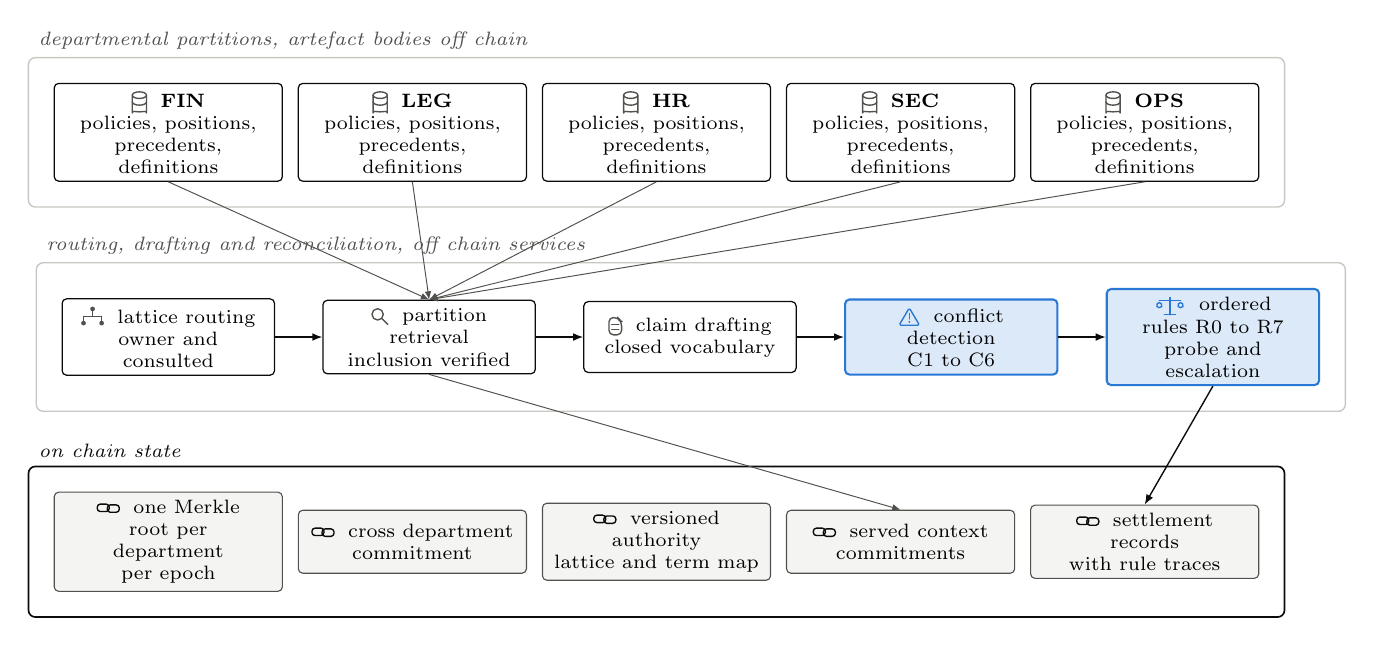
\begin{tikzpicture}[every node/.style={font=\scriptsize}]
  % band 1: partitions
  \foreach \d/\i in {FIN/0, LEG/1, HR/2, SEC/3, OPS/4} {
    \node[bx, text width=27mm, minimum height=9mm] (p\i) at (\i*31mm, 0)
      {\ico{store}{binkb}\; \textbf{\d}\\ policies, positions,\\ precedents, definitions};
  }
  \begin{scope}[on background layer]
    \node[band, fit=(p0)(p4), inner sep=3.2mm] (band1) {};
  \end{scope}
  \node[bandlab, anchor=south west] at ($(band1.north west)+(0.8mm,0.4mm)$)
    {departmental partitions, artefact bodies off chain};

  % band 2: services
  \node[bx, text width=25mm, minimum height=9mm] (s0) at (0,-26mm)
    {\ico{tree}{binkb}\; lattice routing\\ owner and consulted};
  \node[bx, right=6mm of s0, text width=25mm, minimum height=9mm] (s1)
    {\ico{probe}{binkb}\; partition retrieval\\ inclusion verified};
  \node[bx, right=6mm of s1, text width=25mm, minimum height=9mm] (s2)
    {\ico{doc}{binkb}\; claim drafting\\ closed vocabulary};
  \node[bxhi, right=6mm of s2, text width=25mm, minimum height=9mm] (s3)
    {\ico{warn}{bblue}\; conflict detection\\ C1 to C6};
  \node[bxhi, right=6mm of s3, text width=25mm, minimum height=9mm] (s4)
    {\ico{scale}{bblue}\; ordered rules R0 to R7\\ probe and escalation};
  \begin{scope}[on background layer]
    \node[band, fit=(s0)(s4), inner sep=3.2mm] (band2) {};
  \end{scope}
  \node[bandlab, anchor=south west] at ($(band2.north west)+(0.8mm,0.4mm)$)
    {routing, drafting and reconciliation, off chain services};

  \foreach \a/\b in {s0/s1, s1/s2, s2/s3, s3/s4} \draw[flow] (\a) -- (\b);
  \foreach \i in {0,1,2,3,4} \draw[faint] (p\i.south) -- ($(s1.north)+(0,0)$);

  % band 3: on chain
  \foreach \t/\i in {%
      {one Merkle root per\\ department per epoch}/0,
      {cross department\\ commitment}/1,
      {versioned authority\\ lattice and term map}/2,
      {served context\\ commitments}/3,
      {settlement records\\ with rule traces}/4} {
    \node[bxsoft, text width=27mm, minimum height=8mm] (l\i) at (\i*31mm, -52mm)
      {\ico{link}{bink}\; \t};
  }
  \begin{scope}[on background layer]
    \node[band, fit=(l0)(l4), inner sep=3.2mm, draw=bink, line width=0.6pt] (band3) {};
  \end{scope}
  \node[bandlab, anchor=south west, text=bink] at ($(band3.north west)+(0.8mm,0.4mm)$)
    {on chain state};

  \draw[faint] (s1.south) -- (l3.north);
  \draw[flow] (s4.south) -- (l4.north);
\end{tikzpicture}
\caption{Architecture of the proposed framework. Artefact bodies remain off chain.}
\label{fig:architecture}
\end{figure*}

\subsection{Overview, Actors and Assumptions}

The organisation is modelled as a finite set of departments $D=\{d_1,\dots,d_n\}$. Each department maintains a partition and operates one generative agent. Each department also holds a signing key registered on a permissioned EVM compatible ledger. The architectural separation of execution from ordering and validation that such ledgers adopt \cite{androulaki2018fabric} is assumed but not relied upon. Employees issue queries to the framework. A reconciliation service is operated centrally and holds no authority of its own, since every decision it takes is dictated by the registered lattice and by the ordered rules rather than by a model judgement.

Three assumptions bound the scope of the design. First, the claim vocabulary is closed and shared. Departments therefore differ in what they assert rather than in what an assertion can be about. That property makes conflict mechanically detectable and deterministic scoring possible without a model judge \cite{wang2024unfair}. Second, the authority lattice exists as an organisational fact before it is registered, since the proposed framework mechanises an allocation of mandate that the entity already possesses. In a government entity the corresponding instrument is the delegation of authority matrix read together with the terms of reference of each department. Section~VI states what registering that instrument involves. Third, the ledger is permissioned and the ordering service tolerates fewer than one third of participants being compromised under the standard Byzantine fault model \cite{castro2002pbft}, whereas lattice registration additionally requires a quorum of departmental registrars. Under these assumptions, artefact bodies remain off chain. Only commitments, bindings and settlements are written on chain, following the established off-chaining patterns \cite{eberhardt2017offchain}.

\subsection{The Partition and Lattice Components}

The partition component holds and anchors what each department knows. A departmental artefact is the unit of institutional memory and belongs to exactly one department. Every artefact is written once, and it is superseded rather than edited. Each artefact carries an identifier and the owning department. The artefact class is one of policy, position, precedent or definition. Further fields record the body, the policy family and version under which it was issued and the effective window. The claim type and subject it speaks to are recorded, together with the modality and conditions it asserts. Any ordering constraints it imposes are recorded with the signer identity and the attested quality. The ledger derived batch and epoch fields complete the record. A policy is a rule the owning department imposes, whereas a position is what a consulted department holds on a matter it does not own. Positions are retrievable and are the material a consulted agent draws on, and positions never bind.

Anchoring is performed in two stages. In the first stage, each department serialises and hashes its artefacts canonically and signs each leaf with the departmental key. One Merkle root is committed per epoch, which yields logarithmic inclusion proofs at the point of use \cite{merkle1988signature}. In the second stage, a cross department commitment binds the set of departmental roots for that epoch into a single root. The second stage is what prevents a department from silently rewriting its own history in isolation, since a departmental root that is not covered by the cross department commitment for its epoch is inadmissible as evidence during reconciliation. Partitioning is enforced by the settlement contract. That contract accepts an epoch root or a served context commitment for a department only under that department's registered key, which prevents a department from writing into another department's partition. Read permissions follow a role based mapping \cite{sandhu1996rbac}. Superseded artefacts are retained and marked rather than removed, because a settlement made in the past must remain replayable against the artefacts that were in force at the time. Erasure obligations are handled by tombstoning off-chain bodies while retaining the commitment, which preserves the replayability of a settlement without retaining the erased content.

The lattice component declares who is authoritative for what, and it is the element that distinguishes the proposed framework from an ensemble of departmental assistants. The lattice is a versioned object registered on chain and it declares four items. The owner $\mathrm{own}(t)\in D$ of each claim type $t$ in the closed type vocabulary $T$ is the single department whose deontic assertions on $t$ bind. The consulted set $\mathrm{cons}(t)\subseteq D$ lists the departments whose assertions on $t$ are admissible as advisory context and never as obligations. The precedence relation $\succ_s$ is a strict partial order over $D$ for each subject $s$ on which two owners can collide, and it settles contradictions that ownership alone does not decide. Finally, the mandatory flag marks the claim types for which the absence of an owner rule is a defect rather than a silence.

Two conditions are checked at registration and a lattice violating either is refused. The union of the per subject chains must be acyclic as a relation over departments, since a cycle would make deterministic resolution impossible and would return the decision to a model. Additionally, every mandatory claim type must have exactly one owner. The lattice version is recorded in every settlement. A later auditor therefore evaluates a past decision under the mandate that was in force rather than under the current one. Registering the lattice rather than prompting it is the mechanism by which institutional authority remains in the institution, and Section~IV reports what occurs when an adversary is able to write to the registry.

\subsection{The Drafting Component}

The drafting component produces the departmental output. A departmental agent does not return prose but a set of claims, each of which is a structured assertion over the closed vocabulary. Table~\ref{tab:claim} summarises the claim schema. The design has three consequences for reconciliation. Expressing modality explicitly separates a deontic claim from a factual one, and the jurisdiction rule operates on that distinction. A deontic claim carries a modality other than fact. A deontic claim that survives reconciliation with binding status is an obligation, and obligations are the unit that the coverage, spurious rate and attribution measures of Section~IV count. Binding each claim to the policy version of the artefacts that support it makes staleness a property of the claim rather than an inference about it \cite{vu2024freshllms}. Requiring every claim to cite artefacts from the context committed before drafting makes a fabricated citation rejectable rather than merely detectable afterwards, which is the failure mode reported as frequent by Gao et al. \cite{gao2023citations}.

\begin{table}[!t]
\centering
\caption{The departmental claim schema.}
\label{tab:claim}
\footnotesize
\begin{tabular}{@{}>{\raggedright\arraybackslash}p{0.40\columnwidth}>{\raggedright\arraybackslash}p{0.52\columnwidth}@{}}
\toprule
Field & Content \\
\midrule
\texttt{claim\_id} & Stable identifier within the query \\
\texttt{department} & Issuing department \\
\texttt{claim\_type} & Type drawn from the closed type vocabulary $T$ \\
\texttt{modality} & One of must, must\_not, should, should\_not, may, fact \\
\texttt{subject} & Action or object term from the closed vocabulary \\
\texttt{condition} & Conjunction of closed predicate terms \\
\texttt{ordering} & Constraints of the form subject $a$ precedes subject $b$ \\
\texttt{policy\_family} & Policy family the claim is issued under \\
\texttt{policy\_version} & Version of that family \\
\texttt{validity\_window} & Dates between which the claim applies \\
\texttt{citations} & Artefact identifiers, all from the served context \\
\texttt{confidence} & Agent reported confidence in the unit interval \\
\midrule
\texttt{served\_root} & Derived. Commitment to the context served \\
\texttt{status} & Derived. Binding, advisory, context or dropped \\
\texttt{rule\_trace} & Derived. Ordered list of rules applied \\
\bottomrule
\end{tabular}
\end{table}

A query is decomposed into the set $T_q\subseteq T$ of claim types it engages together with the subjects it raises, and routing then follows the lattice, where for each $t\in T_q$ the query is sent to $\mathrm{own}(t)$ and to $\mathrm{cons}(t)$. Each addressed department retrieves from its own partition only. Retrieval verifies the inclusion proof of every candidate artefact against the committed root and commits the served set as a Merkle root before drafting begins. Notably, the served set is not filtered for currency at this stage, because superseded artefacts rank highly on similarity and a framework that never observes them cannot be evaluated on what it does with them. Currency is therefore enforced during reconciliation. The ordering of commitment and drafting is material, since the context is committed first and the claims are produced second, which is what makes the citation of an unserved artefact a detectable protocol violation rather than an assessment of plausibility.

\subsection{The Reconciliation Component}

The reconciliation component detects and settles conflict among the departmental claims. The component is described in four parts. These are the conflict taxonomy and the ordered rules, followed by the completeness probe and the terminal outcomes.

Conflict is defined over claims rather than over passages, which is what allows it to be classified mechanically. Table~\ref{tab:conflicts} states the six classes. Two of those classes deserve further comment. Jurisdiction conflict is the class in which a department asserts an obligation over a claim type it does not own, and it is invisible to a pooled index because pooling discards the department field on which the test depends. Silent omission is the class in which a mandatory claim type receives no assertion from its owner, and it is invisible to any architecture that reasons only over retrieved material, because the defect is the absence of material rather than its content. The literature on knowledge conflict addresses conflicts among present passages \cite{xu2024conflicts} and does not represent either class. Notably, the three level account of syntactic, semantic and pragmatic boundaries \cite{carlile2004transforming} is visible in the taxonomy. C5 is a syntactic and semantic boundary made machine checkable, whereas C1 and C3 are pragmatic boundaries at which the interests of two units differ.

\begin{table}[!t]
\centering
\caption{Classes of cross departmental conflict and the rule that addresses each.}
\label{tab:conflicts}
\footnotesize
\begin{tabular}{@{}>{\raggedright\arraybackslash}p{0.20\columnwidth}>{\raggedright\arraybackslash}p{0.53\columnwidth}>{\raggedright\arraybackslash}p{0.13\columnwidth}@{}}
\toprule
Class & Detection test & Rule \\
\midrule
C1 Contradiction & Two binding claims share a subject, their conditions are jointly satisfiable, and their modalities are incompatible & R3, R4 \\
C2 Precedence & The union of the ordering constraints over the surviving claims contains a cycle & R6 \\
C3 Jurisdiction & A deontic claim of type $t$ is issued by a department other than $\mathrm{own}(t)$ & R2 \\
C4 Staleness & A claim is supported only by artefacts whose effective window does not contain the query date & R1 \\
C5 Definitional & Two claims use the same condition term under departmental definitions that the registered term map does not equate & R7 \\
C6 Omission & A mandatory claim type and subject raised by the query has no rule in force in the owner's partition & R5 \\
\bottomrule
\end{tabular}
\end{table}

Reconciliation is deterministic and its rules are applied in a fixed order. Determinism is not a performance decision, since it is what makes a settlement replayable by an auditor holding only the record and the anchored partitions, and it is what keeps the resolution of an organisational mandate out of a model's discretion. Table~\ref{tab:rules} states the rules, and Figure~\ref{fig:protocol} illustrates the resulting state machine.

\begin{table}[!t]
\centering
\caption{The ordered resolution rules R0 to R7.}
\label{tab:rules}
\footnotesize
\begin{tabular}{@{}>{\raggedright\arraybackslash}p{0.10\columnwidth}>{\raggedright\arraybackslash}p{0.82\columnwidth}@{}}
\toprule
Rule & Action \\
\midrule
R0 & Admissibility. Drop any claim whose citations are not a subset of the served set committed for its department, and any claim citing an artefact whose inclusion proof fails against the committed root \\
R1 & Currency. Drop any claim whose supporting artefacts lie outside their effective window at the query date, and record the drop as a staleness conflict \\
R2 & Jurisdiction projection. For each claim type $t$, retain deontic claims only from $\mathrm{own}(t)$; demote deontic claims from $\mathrm{cons}(t)$ to advisory status and retain their factual claims unchanged \\
R3 & Precedence. For contradictions between departments that both survive R2, resolve by $\succ_s$; if the departments are incomparable under $\succ_s$, escalate the subject \\
R4 & Evidence weight. For contradictions internal to one department, prefer the newer policy version, then the higher attested quality, then the greater citation support; if these are equal, escalate \\
R5 & Completeness probe. For every claim type and subject raised but not settled, query the owner's partition for existence; admit the located rule as a drafted claim and re-apply R3, or, if the type is mandatory and nothing is in force, record an omission for escalation \\
R6 & Ordering. Test the surviving ordering constraints for a cycle; if one exists, escalate that constraint set. No order is emitted, so none has to be canonical \\
R7 & Definitional normalisation. Rewrite condition terms through the registered term map; if a term used by two departments is unmapped, escalate it and withdraw the claims that carry it \\
\bottomrule
\end{tabular}
\end{table}

\begin{figure}[!t]
\centering
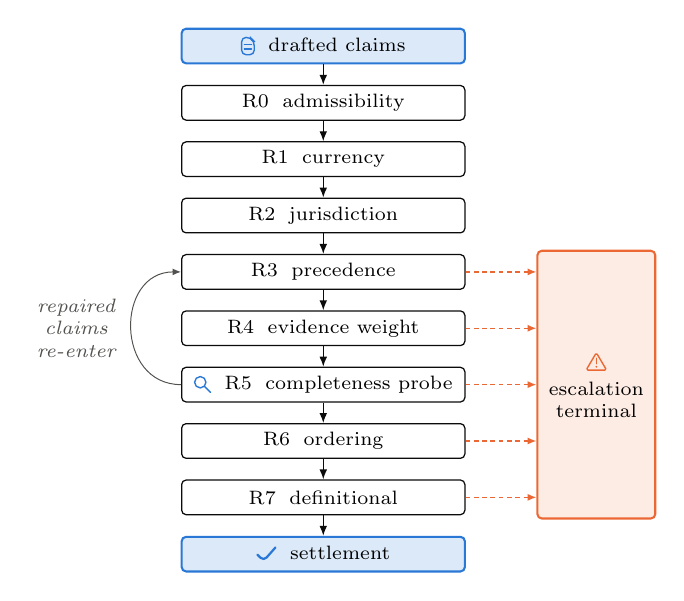
\begin{tikzpicture}[every node/.style={font=\scriptsize}]
  \def\rw{34mm}
  \node[bxhi, text width=\rw, minimum height=4.4mm] (n0) {\ico{doc}{bblue}\; drafted claims};
  \node[bx, below=2.6mm of n0, text width=\rw, minimum height=4.4mm] (n1) {R0\; admissibility};
  \node[bx, below=2.6mm of n1, text width=\rw, minimum height=4.4mm] (n2) {R1\; currency};
  \node[bx, below=2.6mm of n2, text width=\rw, minimum height=4.4mm] (n3) {R2\; jurisdiction};
  \node[bx, below=2.6mm of n3, text width=\rw, minimum height=4.4mm] (n4) {R3\; precedence};
  \node[bx, below=2.6mm of n4, text width=\rw, minimum height=4.4mm] (n5) {R4\; evidence weight};
  \node[bx, below=2.6mm of n5, text width=\rw, minimum height=4.4mm] (n6)
    {\ico{probe}{bblue}\; R5\; completeness probe};
  \node[bx, below=2.6mm of n6, text width=\rw, minimum height=4.4mm] (n7) {R6\; ordering};
  \node[bx, below=2.6mm of n7, text width=\rw, minimum height=4.4mm] (n8) {R7\; definitional};
  \node[bxhi, below=2.6mm of n8, text width=\rw, minimum height=4.4mm] (n9)
    {\ico{check}{bblue}\; settlement};

  \foreach \a/\b in {n0/n1,n1/n2,n2/n3,n3/n4,n4/n5,n5/n6,n6/n7,n7/n8,n8/n9}
    \draw[flow] (\a) -- (\b);

  \node[bxwarn, text width=13mm, minimum height=34mm, right=9mm of n6, anchor=west] (esc)
    {\ico{warn}{borange}\\[2pt] escalation\\ terminal};
  \foreach \s in {n4,n5,n6,n7,n8} \draw[escal] (\s.east) -- (esc.west |- \s);

  \draw[faint] (n6.west) to[out=180,in=180,looseness=1.5] node[left=0.8mm, midway,
      font=\scriptsize\itshape, text=binkb, align=center] {repaired\\claims\\re-enter} (n4.west);
\end{tikzpicture}
\caption{The reconciliation state machine, with escalation as a terminal state.}
\label{fig:protocol}
\end{figure}

The completeness probe at R5 requires its own account, because the evaluation reported in Section~IV indicates that it carries more of the effect than any other rule. Similarity retrieval answers the question of what a partition says about a situation but cannot answer whether a partition says anything at all, since the absence of a passage from a ranked list is not the absence of a rule. Without the probe, R5 must treat every unanswered claim type as a potential organisational gap. Retrieval and drafting both fail some of the time, and the framework then escalates more often than the organisation warrants. Accordingly, the probe is a deterministic lookup on claim type, subject and date against the owning department's own store. That lookup is an ordinary indexed query rather than a similarity search. The probe is available precisely because the claim vocabulary is closed and the partition is identified. The result of the probe is appended to the served commitment for that department before the repaired claim is admitted. Admissibility at R0 therefore continues to hold over the augmented context. Furthermore, the repaired claim is drafted by the owning department under the same conditions as any other claim. Drafting failure therefore applies to the repaired claim as well. Notably, the probe presupposes both the partition and the lattice, since without an owner there is no partition to probe. Section~IV reports a baseline that applies the probe without a lattice in order to isolate that dependency. Three properties of the probe bound what may be concluded from its measured contribution and are stated here rather than left to be inferred. The probe is a closed world existence check. The check is therefore sound only where the owner's partition is complete for its mandatory claim types, which holds by construction in the corpus of Section~IV and does not hold of a real store. The probe reads the claim type, subject and effective window fields that every anchored artefact carries. Those are the fields from which the ground truth of Section~IV is computed. The near perfect detection of omission reported there is therefore a consistency check between two evaluations of the same lookup rather than an independent measurement. Finally, the contribution of the probe is measured against an unfiltered lexical retriever. A retriever that filtered candidates by claim type and effective window before ranking would absorb part of that contribution, and no such variant was evaluated.

The protocol has three terminal outcomes. A full settlement produces an answer in which every obligation is attributed to its owning department and carries the artefacts that support it. A partial settlement produces an answer for the claim types that reconciled together with an escalation for those that did not, which is the common case in practice, since a query typically engages several claim types of which only one is contested. A full escalation produces no advice and instead names the departments, the claim types and the class of conflict that blocked resolution. Accordingly, the proposed framework treats refusal as a designed output rather than as a fallback, which follows the selective prediction position that coverage should be traded explicitly against correctness \cite{kamath2020selective} and the empirical finding that models left unaided recognise their own limits poorly \cite{yin2023knowunknown}.

\subsection{Settlement, Properties and Cost}

The settlement component binds each outcome to the evidence that produced it. Every terminal outcome is written to the settlement registry as an on-chain record. That record binds the query identifier, the lattice version and the per department served roots. The same record binds the hash of the submitted claim set, the detected conflicts with their classes and the ordered rule trace. The outcome type and the hash of the delivered advice complete the record. Accordingly, the registry converts advice into an accountable act. An auditor holding the record and the anchored partitions recomputes the rule trace and obtains the same outcome. Any divergence identifies either a corrupted partition or a protocol violation. The implementation was performed in Solidity (0.8.20) in two contracts. The \texttt{AuthorityLattice} contract holds the versioned mandate and requires a quorum of registrars to register a new version. The \texttt{SettlementRegistry} contract accepts a served context commitment from each department, refuses to settle a query for which a named department has not committed, and exposes a citation admissibility check that verifies a Merkle inclusion proof against the committed served root without consuming storage.

Five properties follow from the construction and are tested in Section~IV rather than asserted. Every deontic clause of a settled answer is attributable to exactly one owning department and to a specific artefact set. A citation that was not served cannot appear in a settled answer, because R0 removes the claim that carries it. A department cannot impose an obligation outside the claim types it owns, because R2 demotes such claims before any contradiction is resolved. Any settlement is replayable and yields the same outcome, because the rules are deterministic and their inputs are committed. Section~IV-F reports the replay that tests this rather than assuming it. Finally, the influence of a captured department is bounded to the claim types it owns together with advisory context elsewhere, because the projection in R2 does not depend on the content the captured department supplies.

Four limits follow with equal force. The lattice registry is a governance single point of failure, since an adversary able to register a lattice version can redirect ownership. The proposed framework mitigates but does not remove this exposure through quorum registration and through recording the lattice version in every settlement, which makes a hostile change visible in retrospect rather than impossible, and Section~IV quantifies the resulting damage. Additionally, collusion between an owner department and a consulted department is not detectable by the protocol, because the protocol reasons about mandate rather than about motive. An owner department that is mistaken is faithfully reproduced, since the proposed framework guarantees attribution rather than correctness, which is a deliberate boundary. Finally, both the mandatory type declarations and the term map must be maintained, since a stale term map converts a definitional conflict into an undetected one.

Whether a ledger is required at all follows the criteria of W\"{u}st and Gervais \cite{wust2018blockchain}, namely several writers that do not trust one another together with the absence of an operator all of them trust. A signed and witnessed append only log would supply tamper evidence, inclusion proofs and the commit before draft ordering on which R0 depends. No measurement reported in Section~IV depends on a chain, since every property tested there is recomputed from signatures and Merkle roots and the gas figures are analytical. The ledger is retained for two reasons that a log operated by one party does not meet. The cross department commitment and the lattice registration are agreements among departments that do not trust the operator of the reconciliation service. The settlement contract refuses at write time to settle a query for which a named department has not committed. The invariant therefore does not rest on that operator's honesty. Accordingly, an organisation that does trust a single operator may replace the ledger by such a log without loss to any result reported here.

The dominant cost is drafting, since each routed department performs its own retrieval and generation. Accordingly, the cost grows with the number of departments the lattice routes to rather than with the size of the organisation, and the lattice is the mechanism that keeps that number small. Reconciliation itself is quadratic in the number of claims within a subject bucket and linear in the number of buckets, whereas the completeness probe adds one indexed lookup per unsettled claim type and subject. On-chain cost is one settlement write per query together with one batch anchoring write per department per epoch. The gas figures reported in Section~IV are analytical rather than chain measured.

\section{Evaluation}

\subsection{Experimental Configuration and Operating Point}

The evaluation was conducted using a generated corpus that models the shared services functions of a mid sized entity. Five functions are modelled over twenty quarters. The first two are finance and the legal and compliance function. The remaining three are human resources, information security and operations. The claim types cover the matters on which those functions issue binding rules. These matters comprise procurement and vendor onboarding, contracting and liability, and sanctions screening. They also comprise payment and budget authority, together with employment and background checks. Data classification and access provisioning are covered, as are incident reporting and service continuity. The closed vocabulary contains 25 claim types of which 14 are mandatory, 38 subjects of which 18 are spoken about by claim types with different owners, and 20 condition predicates of which six carry departmental definitions. The registered lattice provides a precedence chain for ten of the eighteen shared subjects. The remaining eight are subjects on which the organisation has never decided who prevails. Those eight are therefore the subjects on which the proposed framework must escalate rather than choose. Policy families are revised on department specific schedules of two to six quarters in single quarter steps. Version skew therefore arises from the schedule rather than from injection. The generated corpus contains 1082 anchored artefacts. These comprise 361 policies and 367 positions, together with 324 precedents and 30 definitions. The artefacts were signed with Ed25519 keys and hashed as canonical JSON leaves. One Merkle root was committed per department per epoch over fourteen epochs, and a cross department commitment binds the departmental roots of each epoch.

Four hundred scenarios were generated, where a scenario is an employee question that engages several claim types and raises a set of subjects. The generated scenarios engage 2.85 claim types and 2.54 departments on average and carry 3.00 ground truth obligations. Ground truth was computed from the corpus and the lattice alone, without retrieval or agents or any system under test. The ground truth states for each scenario the reconciled obligation set and the attribution of each obligation. The same ground truth states whether the organisation holds a reconciled position at all. Of the 400 scenarios, 190 admit no reconciled position on at least one matter. The distribution is 90 contradictions and 84 definitional conflicts, together with 61 omissions and 23 precedence cycles. Each figure counts the number of scenarios carrying a conflict of that class. Table~\ref{tab:detection} instead counts distinct conflict instances, of which several are raised by more than one scenario, which is why the definitional support there is 78 rather than 84.

The implementation was performed using Python (3.11), and the figures were produced using matplotlib (3.10) and the departmental signatures were produced using the cryptography library (46.0). Every system employs the same BM25 retriever with $k=24$ artefacts per partition. The pooled systems receive $k$ multiplied by the number of routed partitions, which gives both arrangements the same served volume. Scoring was performed by deterministic set comparison over the closed vocabulary, and no model judge was employed at any point, which avoids the documented biases of such judges \cite{wang2024unfair}. Significance was assessed by paired bootstrap with ten thousand resamples together with a paired two sided randomisation test. Sixteen comparisons were performed in total. A Bonferroni corrected threshold of $0.003125$ was therefore applied wherever a comparison is described as surviving correction. The complete implementation, the corpus generator and the model returns are released with the results in the accompanying artefact under the global seed 20260902. A data card states which quantities are measurements and which follow from the construction of the corpus.

Seven architectures are compared and are labelled B0 to B5 in Table~\ref{tab:systems}. B0 drafts an answer without any retrieval. B1 drafts over a single pooled index from which departmental provenance has been discarded, and B2 is the same arrangement with the department field of each served artefact retained. B3 routes the query to every department, drafts in each partition and concatenates the departmental claim sets without reconciliation. B3P adds the completeness probe to B3 without a lattice, in order to isolate the dependency noted in Section~III-D. B4 passes the concatenated departmental claims to a referee that selects among them by the evidence available inside the exchange, without access to a registered mandate. B5 denotes the proposed framework in full. Two further arms were added after review, because the six above are not matched to the proposed framework on the affordances that an ordinary enterprise index possesses. B2F is B2 given an effective window currency filter applied at retrieval and an exact metadata lookup for a raised pair the ranked list did not surface, which are the two affordances the proposed framework obtains from R1 and from the completeness probe, and it has no lattice. B4A is B4 given an abstention state. Where two departments assert incompatible modalities on one subject the referee declines that subject rather than selecting a winner, which is the mechanism the selective prediction literature describes \cite{kamath2020selective}. Accordingly, the comparison is against baselines that can filter and look up and refuse. Baselines denied those capacities are not the point of comparison. Two falsification conditions were fixed before the experiments were run and are reported either way. If B2 had matched B5 on jurisdiction violations, provenance visibility alone would suffice and the lattice would be unnecessary. If B4 had matched B5 on attribution and on escalation, a referee would suffice.

The departmental agent was simulated by a generator with six failure modes. These correspond to failures documented for language models grounded in retrieved context. The first three modes are omission of supported content, unsupported assertion and modality drift. The remaining three are reliance on superseded material, citation of unserved material and assertion outside the agent's own mandate. The rates of these modes are scaled by a single parameter $\lambda$, and every headline result is accompanied by a sweep over $\lambda$ rather than being reported only at one assumed point.

The operating point itself was fixed by placing a language model in the loop, namely \texttt{claude-opus-5}. That model also constructed the harness, wrote the generator and analysed the results. The resulting conflict of interest is addressed in Section~V. Ten scenarios were sampled and stratified by the conflict classes they contain. For each scenario the departments routed by the lattice were given a prompt containing the situation and the claim types they were asked about with their owned or consulted role. The prompt also served ten artefacts from their own partition, which is a smaller and therefore less superseded context than the twenty four the simulated agent works with. Ground truth appeared in no prompt. The model returned 51 claims across 38 prompts, all of which were schema valid, and produced no instance of any of the six failure modes. Accordingly, that measurement bounds the rates from above rather than estimating them. With zero events the ninety five per cent Wilson upper bounds are 0.070 on the four rates estimated over all 51 claims and 0.088 on mandate overreach over 40 opportunities. The bound on modality drift is 0.259, which had only 11 opportunities and falls below the threshold of twenty opportunities applied here. Notably, the exclusion is what makes the fitting rule satisfiable, since no grid point reaches 0.259 on that mode. Section~IV-E therefore reports a separate run in which the modality base rate alone is raised until that bound is met. The operating point $\lambda^\star=0.6$ is the smallest grid value whose failure vector lies at or above every usable upper bound, where the binding constraint is citation fabrication, which requires $\lambda\ge0.583$. The headline results are therefore reported at a point at which the simulated agent lies at or above the upper bound on every mode with at least twenty opportunities. The margin is marginal on citation fabrication and a factor of between 1.7 and 2.6 on the others, which is the conservative direction. Modality drift is not covered by that bound. The returns are released verbatim in the accompanying artefact.

\subsection{Corpus Characterisation and Retrieval}

Figure~\ref{fig:corpus} reports the distribution of organisational conflict across the four classes that arise from the corpus rather than from the agent, together with two measures of version skew. The second panel is the more consequential of the two. Eighteen policy families are maintained on five different revision schedules. The organisation therefore sits at up to five different revision generations at the same moment, rising from one generation in the first year to five by the seventeenth quarter. More consequentially, between 0.831 and 0.845 of the policy corpus is superseded at any given quarter and remains retrievable. A superseded rule is retained rather than deleted, which keeps past settlements replayable. A retriever that ranks by similarity has no reason to prefer the small share of the corpus that is current. The measured share of superseded material in the served set is 0.808 for the partitioned arrangement and 0.834 for the pooled arrangement. Both figures are almost exactly the share present in the corpus itself. Accordingly, staleness is an organisational property in this setting rather than a model defect, which is the reason R1 exists.

\begin{figure*}[!t]
\centering
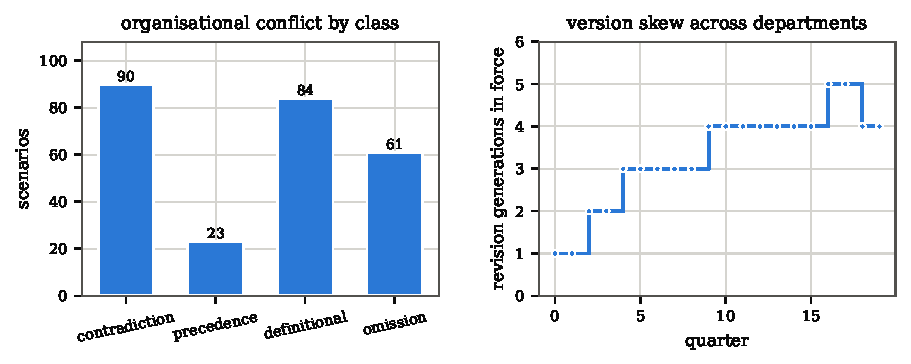
\includegraphics[width=\textwidth]{figures/fig4_corpus.pdf}
\caption{Corpus characterisation. Left, organisational conflict by class. Right, version skew.}
\label{fig:corpus}
\end{figure*}

Two of the six conflict classes cannot be represented by a pooled architecture at all. Jurisdiction overreach is a statement about which department is entitled to issue a claim, and no pooled arrangement registers an owner against which that entitlement can be tested. Silent omission is a statement about the absence of a rule, whereas no architecture that reasons only over retrieved passages can distinguish absence from non retrieval. A third class, namely precedence, requires ordering constraints attributable to distinct departments and is therefore also unavailable to a pooled index. In answer to RQ1, roughly half of the generated scenarios contain a conflict that the organisation has not resolved, and half of the conflict classes are structurally invisible to the standard enterprise deployment.

Figure~\ref{fig:retrieval} reports retrieval quality, and the result runs against the proposed framework. At equal served volume, pooled retrieval recovers the owning department's rule for 0.983 of the required claim type and subject pairs, whereas partitioned retrieval recovers 0.901. Pooled nDCG@10 is 0.340 against 0.209 for the partitioned arrangement. Partitioning is therefore worse at retrieval, and the reason is straightforward. A pooled index can spend its whole budget on whichever partition is most relevant, whereas partitioning spends a fixed budget in each routed partition whether or not that partition has much to say. Additionally, the share of served artefacts that are superseded is high and similar in both arrangements, namely 0.808 and 0.834. This result is material for the interpretation of the remaining experiments, since the gains reported below are not attributable to retrieving better but to what is done with what was retrieved and to the completeness probe, which is a lookup rather than a search.

\begin{figure}[!t]
\centering
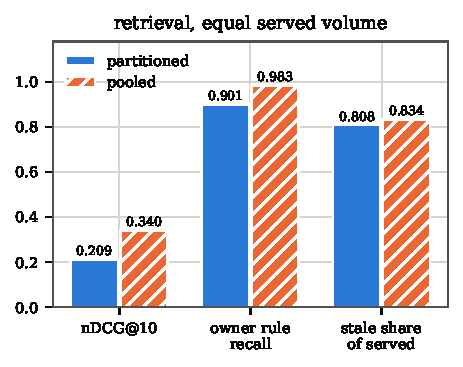
\includegraphics[width=\columnwidth]{figures/fig5_retrieval.pdf}
\caption{Retrieval at equal served volume, partitioned against pooled.}
\label{fig:retrieval}
\end{figure}

\subsection{Composite Guidance}

Table~\ref{tab:systems} reports the comparison across the seven architectures and the two affordance matched arms defined in Section~IV-A, at $\lambda^\star$. Five observations follow from the comparison.

\begin{table*}[!t]
\centering
\caption{System comparison at $\lambda^\star=0.6$ over 400 scenarios.}
\label{tab:systems}
\footnotesize
\setlength{\tabcolsep}{3.5pt}
\begin{tabular}{@{}lccccccccc@{}}
\toprule
System & Coverage & Spurious & Attribution & Jurisdiction & Citation & Stale & Silent wrong & Escalation & Obligations \\
 & & rate & & violation & validity & obligations & answer & P / R & emitted \\
\midrule
B0 no retrieval                & 0.702 & 0.788 & 0.000 & 0.000 & 0.000 & 0.000 & 0.916 & n/a & 10.48 \\
B1 pooled                      & 0.286 & 0.811 & 0.000 & 0.000 & 1.000 & 0.741 & 0.853 & n/a & 4.79 \\
B2 pooled with labels          & 0.286 & 0.811 & 0.454 & 0.546 & 1.000 & 0.741 & 0.853 & n/a & 4.79 \\
B3 departmental, concatenated  & 0.420 & 0.787 & 0.425 & 0.575 & 0.937 & 0.279 & 0.890 & n/a & 6.41 \\
B3P departmental with probe    & 0.497 & 0.774 & 0.477 & 0.524 & 0.907 & 0.252 & 0.890 & n/a & 7.05 \\
B4 departmental with referee   & 0.429 & 0.757 & 0.481 & 0.519 & 0.934 & 0.299 & 0.884 & n/a & 5.81 \\
\midrule
B2F pooled, filtered, lookup   & 0.706 & 0.617 & 0.651 & 0.349 & 0.951 & 0.000 & 0.774 & n/a & 5.69 \\
B4A referee with abstention    & 0.343 & 0.726 & 0.499 & 0.495 & 0.937 & 0.304 & 0.126 & 0.482 / 0.842 & 4.30 \\
\midrule
\textbf{B5 proposed framework} & \textbf{0.870} & \textbf{0.237} & \textbf{1.000} & \textbf{0.000} & \textbf{1.000} & \textbf{0.000} & \textbf{0.100} & 0.904 / 0.890 & 3.47 \\
\bottomrule
\end{tabular}

\vspace{2pt}
\footnotesize\raggedright
Coverage is the share of ground truth obligations emitted with the correct modality, whereas the spurious rate is the share of emitted obligations the organisation does not hold. Attribution is the share ascribed to the owning department, and jurisdiction violation the share ascribed to a department that does not own the matter. Silent wrong answer is the share of scenarios needing escalation that were answered with an assertion on a contested matter. Escalation precision and recall are reported at scenario level, and every rate is rounded to three decimals. B2F and B4A are the affordance matched arms defined in Section~IV-A; their values at the noise realisation of this table lie within the three seed ranges reported in Section~IV-C.
\end{table*}

First, provenance visibility alone changes nothing about what is asserted. B1 and B2 are identical on coverage and spurious rate, and also on citation validity and staleness. The two differ only in that B2 is able to name a department. Presenting the department field to the generator does not cause the generator to respect the mandate, since 0.546 of its obligations are issued in the name of a department that does not own the matter. Accordingly, the first falsification condition stated in Section~IV-A is answered, since provenance visibility does not suffice.

Second, a referee model is not a substitute for a registered mandate. B4 improves attribution over B3 from 0.425 to 0.481 and reduces the spurious rate from 0.787 to 0.757, whereas it leaves the silent wrong answer rate at 0.884 against 0.890. A referee selects among departmental claims by the evidence available inside the exchange, which does not include the question of who is entitled to decide. Accordingly, the second falsification condition stated in Section~IV-A is answered.

Third, the proposed framework attains 0.870 coverage against 0.497 for the strongest grounded baseline B3P. The ungrounded B0 reaches 0.702 only by emitting 10.48 obligations per scenario at a spurious rate of 0.788. The paired difference over B3P is 0.368 with a bootstrap interval of $[0.328,0.408]$ and $p\le10^{-4}$, whereas the spurious rate falls from 0.774 to 0.237, a difference of $-0.537$ with interval $[-0.565,-0.509]$. Every emitted obligation is attributed to its owner and none is issued outside a mandate, both by construction of R2 and by measurement. Citation validity is exactly 1.000 because R0 removes any claim citing material outside the committed served set, whereas the stale obligation rate is exactly 0.000 because R1 removes any claim resting on a superseded artefact. Additionally, the proposed framework asserts less. The framework emits 3.47 obligations per scenario against 6.41 for concatenation and 10.48 for the model without retrieval. That result reproduces at the level of obligations the finding that an ungrounded model proposes a long and largely unsupported plan.

Fourth, and most consequentially, the silent wrong answer rate falls from 0.890 to 0.100. That paired difference is $-0.790$ with interval $[-0.847,-0.732]$ and $p\le10^{-4}$. All sixteen tested contrasts have $p\le10^{-4}$, which is the resolution of ten thousand resamples, and survive Bonferroni correction. The remaining contrasts in this subsection are B4 against B3 and B2 against B1, both of which are descriptive and were not tested. Fifth, and most consequentially for how the four findings above should be read, the two affordance matched arms show that no single advantage of the proposed framework survives in isolation. B2F is the pooled arrangement given the currency filter and the existence lookup. That arrangement raises coverage from 0.286 to 0.706 and removes stale obligations entirely. The gain is more than half of the coverage separation previously attributed to the framework, and it establishes that those two affordances rather than the lattice carry that part of the effect. However, B2F issues 0.349 of its obligations in the name of a department that does not own the matter. The same arrangement asserts 0.617 of them without organisational support and answers confidently on 0.774 of the matters the organisation has not settled. B4A is the referee given an abstention state. That arrangement very nearly matches the proposed framework on the quantity that matters most for safety, at 0.126 against 0.100. B4A purchases that result by surrendering coverage to 0.343 and by escalating at a precision of 0.482, which is to say that it refuses roughly twice as often as the organisation requires. Accordingly, each affordance matched arm attains one of the three properties and forfeits the others. The proposed framework is the only arrangement measured that holds coverage, refusal and attribution together. Attribution is the property neither arm approaches, at 0.651 and 0.499 against 1.000.

Every quantity reported in this subsection was recomputed over five independent agent noise realisations on the same corpus and the same scenarios. Across those five, the coverage of the proposed framework has a mean of 0.877 with a range of 0.017. The coverage of the strongest grounded baseline has a mean of 0.497 with a range of 0.047. The separation of 0.380 therefore exceeds the wider of the two ranges by a factor of eight. Notably, attribution and citation validity have a range of exactly 0.000 across all five realisations. The jurisdiction violation rate and the stale obligation rate behave in the same way. That is the empirical form of the statement that they follow from R0 and R2 by construction rather than from any particular draw. Escalation precision is the least stable quantity reported in this paper, with a mean of 0.913 and a range of 0.061. The value of 0.904 should therefore be read with that width in mind.

In answer to RQ2, departmental partitioning under a registered lattice improves both what is asserted and which department is accountable for it. The coverage component of that improvement is substantially smaller than a comparison against baselines denied a currency filter and an existence lookup would suggest, at 0.164 over B2F rather than 0.373 over B3P. What the lattice supplies and no affordance supplies is attribution and the projection that follows from it. Additionally, the coverage loss that the anticipated design trade predicted did not materialise, because the completeness probe more than compensates for the retrieval loss reported in Section~IV-B. Notably, the ground truth is computed from the corpus and the lattice by the same function the proposed framework approximates, as Section~V states. These differences therefore measure how much of a lattice defined truth each architecture recovers from identical evidence rather than how often the guidance of a real organisation would be correct.

\subsection{Conflict Detection and Escalation Calibration}

Table~\ref{tab:detection} reports detection by class. Omission is detected almost perfectly at 0.984 recall and 1.000 precision, which is the completeness probe performing the function for which it was introduced. Staleness is detected at 0.951 recall. However, contradiction is detected at 0.856 recall and only 0.470 precision, and definitional conflict at only 0.590 recall. These two results are the weakest reported in this paper and both have the same cause, since a contradiction is visible only when both sides survive as binding claims. Accordingly, an agent that omits one side conceals the conflict, whereas a spurious claim with an arbitrary modality manufactures one that does not exist. The 18 falsely escalated scenarios carry 28 falsely escalated conflicts. Of those, 11 are contradictions and 16 are definitional, and one is a precedence cycle. Notably, jurisdiction overreach is detected with perfect precision and only 0.549 recall, because an overreaching claim that fails admissibility or currency is dropped before R2 is able to label it. The proposed framework therefore prevents the harm without recording that it occurred.

\begin{table}[!t]
\centering
\caption{Conflict detection by class at $\lambda^\star$.}
\label{tab:detection}
\footnotesize
\begin{tabular}{@{}llrrr@{}}
\toprule
Class & & Recall & Precision & Support \\
\midrule
C1 & contradiction & 0.856 & 0.470 & 90 \\
C2 & precedence    & 0.739 & 0.944 & 23 \\
C3 & jurisdiction  & 0.549 & 1.000 & 377 \\
C4 & staleness     & 0.951 & 0.833 & 1261 \\
C5 & definitional  & 0.590 & 0.742 & 78 \\
C6 & omission      & 0.984 & 1.000 & 61 \\
\bottomrule
\end{tabular}

\vspace{2pt}
\footnotesize\raggedright
Support is the number of ground truth instances. C1, C2, C5 and C6 are organisational and come from the corpus, whereas C3 and C4 are agent induced and come from the agent log.
\end{table}

Of the 400 scenarios, 190 require escalation. The proposed framework escalates 187 scenarios, of which 169 are correct. That gives a scenario level precision of 0.904 and a recall of 0.890, with 21 misses and 18 false alarms. At the level of individual conflicts rather than scenarios, precision is 0.877 and recall is 0.794. The proposed framework settles 0.533 of scenarios fully, answers 0.460 partially with an escalation attached, and refuses entirely on 0.008. None of the six original baselines escalates at all, which is not a deficiency of tuning but of representation, since none has a state in which the appropriate output is a refusal. The affordance matched arm B4A does have such a state, and the comparison against it is the informative one, since it escalates with a recall of 0.842 at a precision of 0.482 against 0.890 and 0.904 for the proposed framework. Accordingly, a referee that declines wherever it can see disagreement identifies most of the matters that require escalation and is wrong about half of the times it refuses, because visible disagreement between two departments is not the same fact as the absence of a registered order between them.

Notably, the anticipated trade of coverage for safety did not appear in the predicted direction for the proposed framework. Coverage rose rather than fell, by 0.449 over concatenation, whereas the silent wrong answer rate fell by 0.790. The trade does appear for B4A, which surrenders 0.086 of coverage against B4 to obtain its abstention state, which suggests that the trade is a property of refusing without a mandate rather than of refusing as such. What the proposed framework gives up instead is the appearance of completeness, since it answers fully on barely half of the scenarios and attaches an escalation to most of the remainder. In answer to RQ3, escalation is well calibrated at the operating point and materially better calibrated than abstention bolted onto a system without a mandate. The residual 0.100 of scenarios on which the proposed framework still asserts a position the organisation has not settled is the remainder. That remainder arises where a conflict was never detected because one side of it was never drafted.

\subsection{Sensitivity, Adversarial Behaviour, Cost and Scaling}

Figure~\ref{fig:sweep} sweeps the agent failure rate from a perfect agent to a rate several times the upper bound measured from the model in the loop. The separation between the proposed framework and every baseline is preserved across the whole range. Across the sweep, the coverage of the proposed framework falls from 0.978 to 0.806 as the agents degrade. Its spurious rate rises from 0.151 to 0.278 and its silent wrong answer rate rises from 0.063 to 0.111. The retrieval baselines remain between 0.81 and 0.90 on the last of these throughout, whereas the baseline without retrieval remains at 0.92. Escalation precision is essentially flat, between 0.891 and 0.926. The reported advantage is therefore not a product of the chosen operating point, and the proposed framework degrades gradually rather than abruptly as the drafting agents become less reliable. However, the sweep cannot address the definitional component of the advantage identified in Section~V, since the ground truth is unchanged across $\lambda$.

The sweep scales all six failure modes together, whereas one of them is not bounded by the operating point at all. Modality drift had eleven opportunities in the model in the loop sample. Its ninety five per cent upper bound is therefore 0.259. The simulated rate at $\lambda^\star$ is 0.090, which no value on the grid raises to that bound. Accordingly, a separate run was performed in which the modality base rate alone was raised from 0.15 to 0.437. The simulated rate then reaches 0.262 and the bound is met. Under that condition the coverage of the proposed framework falls from 0.892 to 0.710 and its spurious rate rises from 0.221 to 0.395, whereas the silent wrong answer rate rises from 0.095 to 0.137 and contradiction detection falls to 0.465 precision at 0.733 recall. The strongest grounded baseline moves far less, from 0.501 to 0.474, since an arrangement that does not project claims against a mandate is largely indifferent to the modality those claims carry. Notably, modality drift is therefore both the failure mode to which the proposed framework is most exposed and the one mode the operating point does not bound, and the margin over that baseline narrows from 0.391 to 0.236 rather than closing. Omission detection is unaffected at 1.000 precision and 1.000 recall, which is consistent with the probe being a lookup on the artefact record rather than a judgement about a drafted claim.

\begin{figure*}[!t]
\centering
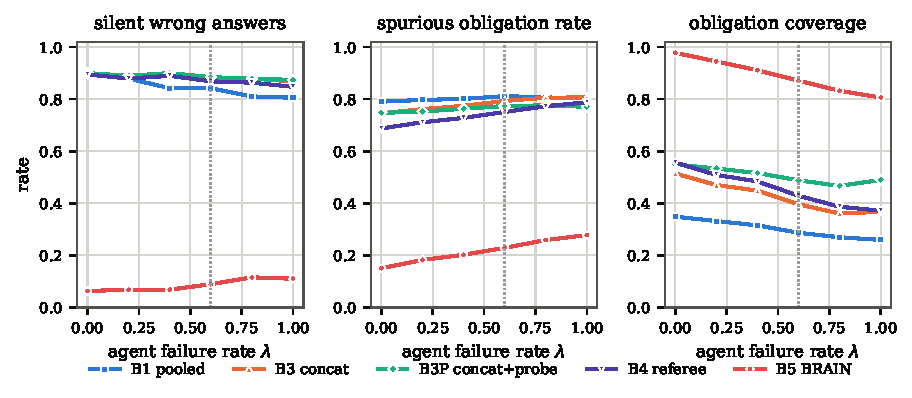
\includegraphics[width=\textwidth]{figures/fig9_sweep.pdf}
\caption{Sensitivity to the agent failure rate $\lambda$. The dotted line marks $\lambda^\star$.}
\label{fig:sweep}
\end{figure*}

Table~\ref{tab:adversarial} reports the five attacks tested. A captured departmental agent that asserts obligations on every matter it is consulted on achieves nothing, since jurisdiction violations remain at 0.000 and neither coverage nor the spurious rate deteriorates, because R2 projects the captured department's deontic claims to advisory status before any contradiction is resolved. Accordingly, the reach of a compromised department is bounded to what that department owns, which is the property the design claimed. Notably, coverage in fact rises to 0.889 and 0.903 and the spurious rate falls to 0.223 and 0.213, because the captured agent was modelled as asserting outside its mandate rather than as omitting inside it. What a captured owner department asserts within its own mandate is the third limit stated in Section~III-E and was not attacked.

Corpus poisoning is more damaging and remains survivable. Forty adversarial artefacts were injected into the security partition, constructed to rank highly and to prohibit what the organisation requires. Those artefacts reduce the coverage of the proposed framework from 0.870 to 0.828 and raise its spurious rate from 0.237 to 0.290. The same injection reduces pooled retrieval coverage to 0.264 with a spurious rate of 0.827 and leaves 0.842 of the scenarios needing escalation answered anyway. Raising citation fabrication and stale exploitation to 0.9 leaves the coverage of the proposed framework at 0.882 and 0.903 and its spurious rate at 0.167 and 0.162, because R0 and R1 discard exactly those claims and the completeness probe then supplies the rule that the discarded claim would have carried, whereas concatenation under the same attack answers wrongly on 0.900 of the scenarios that require escalation.

However, the registry is the exception. An adversary able to register a lattice version that reassigns ownership to a captured department drives attribution from 1.000 to 0.793, jurisdiction violations from 0.000 to 0.204, coverage from 0.870 to 0.595 and escalation precision from 0.904 to 0.580. In answer to RQ4, the proposed framework is robust to compromised agents and poisoned partitions. The same robustness holds against fabricated citations and stale exploitation. The proposed framework is not robust to a compromised mandate. This is the expected conclusion for a design that deliberately relocates authority into a registry, and it is the reason the contract requires quorum registration and the reason every settlement records the lattice version under which it was decided.

\begin{table}[!t]
\centering
\caption{The proposed framework under adversarial conditions.}
\label{tab:adversarial}
\scriptsize
\setlength{\tabcolsep}{3.5pt}
\begin{tabular}{@{}lcccc@{}}
\toprule
Condition & Coverage & Spurious & Jurisd. & Silent \\
\midrule
no attack                        & 0.870 & 0.237 & 0.000 & 0.100 \\
captured SEC agent               & 0.889 & 0.223 & 0.000 & 0.100 \\
captured LEG agent               & 0.903 & 0.213 & 0.000 & 0.095 \\
poisoned partition, prop. & 0.828 & 0.290 & 0.000 & 0.132 \\
poisoned partition, pooled       & 0.264 & 0.827 & 0.000 & 0.842 \\
poisoned partition, concat. & 0.412 & 0.788 & 0.580 & 0.884 \\
citation fabrication, prop. & 0.882 & 0.167 & 0.000 & 0.111 \\
citation fabrication, concat.    & 0.441 & 0.775 & 0.574 & 0.900 \\
stale exploitation, prop. & 0.903 & 0.162 & 0.000 & 0.100 \\
stale exploitation, concat.      & 0.360 & 0.813 & 0.550 & 0.900 \\
\textbf{hostile lattice}         & \textbf{0.595} & \textbf{0.417} & \textbf{0.204} & \textbf{0.137} \\
\bottomrule
\end{tabular}
\end{table}

The proposed framework serves 94.4 artefacts per query against 120.0 for the arrangements that address every department, because the lattice routes only to the owner and the consulted departments of the claim types a query engages, which is 3.9 of the five partitions on average at $k=24$ rather than all five. End to end processing costs 5.7 milliseconds per scenario on a single core against 10.2 for concatenation. Retrieval is the larger part, since pooled retrieval alone costs 5.1 milliseconds. The cost is flat in the number of scenarios, which confirms that it grows with the routed breadth rather than with the corpus history. Scaling the organisation from two to five departments raises the served artefacts from 43.7 to 94.0 and the end to end time from 3.0 to 9.2 milliseconds. That growth is close to linear in the number of departments. Coverage falls from 0.921 to 0.851 and the spurious rate rises from 0.120 to 0.237, which shows that breadth costs accuracy as well as time. Figure~\ref{fig:cost} illustrates these three cost quantities. Notably, the department scaling runs rebuild the corpus and do not benefit from the memoised retrieval of the headline runs, which is why their absolute times exceed the 5.7 milliseconds reported for the same five department configuration above.

\begin{figure*}[!t]
\centering
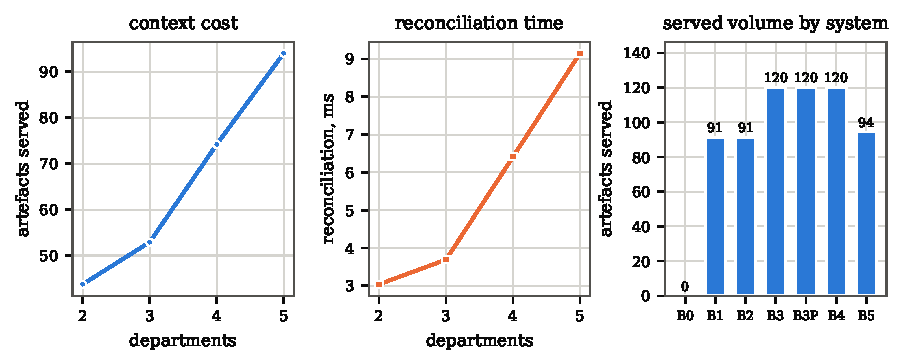
\includegraphics[width=\textwidth]{figures/fig12_cost.pdf}
\caption{Cost: context, reconciliation time and served volume.}
\label{fig:cost}
\end{figure*}

The on-chain cost is analytical rather than chain measured. A settlement writing eight new storage slots with a three topic event costs approximately 186{,}852 gas under the standard opcode schedule. One departmental epoch anchor costs approximately 41{,}512 gas. At five departments and fourteen epochs the anchoring cost is amortised over the whole corpus. The marginal on-chain cost of the proposed framework is therefore one settlement per query. However, the contracts have not been audited and no test network deployment was performed. These figures should therefore be read as an order of magnitude rather than as a measurement.

\subsection{Ablation, Cold Start and Summary}

Table~\ref{tab:ablation} reports the removal of one rule at a time. The differences should be read against a seed noise floor rather than as exact quantities, since the ablation set was repeated over three noise realisations and the widest range observed for any single configuration is 0.038 on coverage and 0.084 on the silent wrong answer rate. Accordingly, the coverage effects of currency and jurisdiction projection exceed that floor and are interpretable, as do those of precedence and the completeness probe. The effects of admissibility and evidence weight do not exceed the floor, and neither do those of the omission record and ordering synthesis. Those four should be read as no measured effect on coverage. On the silent wrong answer rate the interpretable effects are currency, the probe, definitional normalisation and escalation. The completeness probe is by far the largest single contributor relative to unfiltered lexical retrieval, since without it the coverage falls from 0.888 to 0.414 and the escalation precision falls from 0.909 to 0.504, because the proposed framework then treats every retrieval miss as an organisational gap. Currency is the second largest contributor, since without R1 the spurious rate almost doubles from 0.224 to 0.427, the stale obligation rate rises from 0.000 to 0.348 and the silent wrong answers rise from 0.095 to 0.253. Removing jurisdiction projection reintroduces jurisdiction violations at 0.105 and raises the spurious rate to 0.298. Removing escalation entirely raises silent wrong answers from 0.095 to 0.700 while barely changing coverage, which is the clearest statement of the function escalation performs, since it does not improve the answers and it prevents the system from asserting where the organisation has not decided. Finally, removing admissibility affects only citation validity, which falls from 1.000 to 0.961. A fabricated citation rarely changes the modality of the claim that carries it. The check therefore matters for accountability rather than for accuracy. Removing definitional normalisation is the second largest safety effect in the table, since it raises coverage to 0.905 and escalation precision to 0.953 while raising silent wrong answers from 0.095 to 0.247, because an unmapped term then withdraws no claim and triggers no escalation.

\begin{table}[!t]
\centering
\caption{Ablation of the reconciliation rules.}
\label{tab:ablation}
\footnotesize
\begin{tabular}{@{}lccccc@{}}
\toprule
Variant & Coverage & Spurious & Silent & Esc. P & Cit. \\
\midrule
full                       & 0.888 & 0.224 & 0.095 & 0.909 & 1.000 \\
$-$R0 admissibility        & 0.886 & 0.234 & 0.095 & 0.909 & 0.961 \\
$-$R1 currency             & 0.766 & 0.427 & 0.253 & 0.772 & 1.000 \\
$-$R2 jurisdiction         & 0.842 & 0.298 & 0.116 & 0.814 & 1.000 \\
$-$R3 precedence           & 0.834 & 0.232 & 0.090 & 0.761 & 1.000 \\
$-$R4 evidence weight      & 0.887 & 0.225 & 0.090 & 0.919 & 1.000 \\
$-$R5 completeness         & 0.888 & 0.224 & 0.100 & 0.883 & 1.000 \\
$-$completeness probe      & 0.414 & 0.359 & 0.011 & 0.504 & 1.000 \\
$-$R6 ordering             & 0.888 & 0.224 & 0.095 & 0.907 & 1.000 \\
$-$R7 definitional         & 0.905 & 0.266 & 0.247 & 0.953 & 1.000 \\
$-$escalation              & 0.904 & 0.319 & 0.700 & n/a   & 1.000 \\
\bottomrule
\end{tabular}

\vspace{2pt}
\footnotesize\raggedright
The full row uses this experiment's own noise realisation and therefore differs from Table~\ref{tab:systems} by less than the seed range reported in Section~IV-C.
\end{table}

Two properties of the rule set were tested rather than argued. Replayability was exercised by recomputing every settlement from the same committed inputs. The obligations, the attribution and the supporting citations were compared, together with the escalations and the rule trace. The comparison agreed on all 400 scenarios. The hash of the whole advice set is additionally stable across an independent rebuild of the corpus from the global seed. Notably, R6 tests the surviving ordering constraints for a cycle and does not emit an order. Replay therefore requires no ordering convention.

Two corrections to the rule order were then implemented and measured rather than adopted on argument. Restricting the definitional test to a shared subject is the scope the contradiction test already uses. That restriction raises its precision to 1.000 and collapses its recall from 0.590 to 0.077. The silent wrong answer rate more than doubles from 0.100 to 0.232. Evaluating the unmapped term test before the contradiction test rather than after it lowers its recall to 0.192 at a precision of 0.536 and raises silent wrong answers to 0.211, because at that position the surviving claim set has not yet been consolidated by precedence and evidence weight. Accordingly, both variants trade a large loss of definitional recall for precision or for ordering purity, and the order as implemented is retained on the evidence rather than by default. Furthermore, the definitional test operates on the binding set produced by R2, which contains only the deontic claims of owning departments. An advisory claim from a consulted department therefore cannot withdraw an owner's claim.

Cold start was evaluated by deleting the operations partition for the first fifteen quarters. A department then exists on the lattice with nothing anchored behind it. In that period the proposed framework attains 0.901 coverage on what remains, escalates with a precision of 0.971 and a recall of 0.955, and asserts a position on a contested matter in only 0.023 of the cases that require escalation. Accordingly, a department with no record produces escalations rather than fabrications, which is the behaviour a newly created unit requires.

Overall, the four research questions are answered as follows. Roughly half of the generated cross departmental scenarios contain a conflict the organisation has not resolved, and half of the conflict classes cannot be represented by a pooled index at all. Departmental partitioning under a registered lattice raises coverage from 0.497 to 0.870 and reduces the spurious rate from 0.774 to 0.237 with complete attribution, whereas partitioning by itself makes retrieval worse and the gain is attributable to the rules and the probe that follow it. Escalation is calibrated at 0.904 precision and 0.890 recall, with a residual silent wrong answer rate of 0.100. Finally, on the generated corpus the proposed framework withstands a captured consulted department and a poisoned partition, as well as forged or stale evidence. The proposed framework does not withstand a compromised registry. A captured owner department asserting wrongly inside its own mandate was not attacked.

\section{Threats to Validity}

Construct validity is threatened first by the closed vocabulary. Expressing departmental positions as typed claims makes conflict detectable and simultaneously excludes forms of disagreement that resist typing, such as a difference of risk appetite that both departments would express as the same obligation with different urgency. The evaluation therefore measures a well posed subset of organisational disagreement rather than organisational disagreement in general. Additionally, the closed vocabulary is what makes the completeness probe possible. The probe is the largest single contributor to the reported gain relative to unfiltered lexical retrieval. An organisation whose claim types and subjects are not enumerable would therefore obtain a weaker version of the proposed framework than the one measured here. Accordingly, the ablation without the probe reaches 0.414 coverage and should be read as an indication rather than a bound for that case. That ablation retains the closed vocabulary detection tests which such an organisation would also lose. Finally, deterministic scoring over closed vocabularies measures whether the correct terms were emitted rather than whether the resulting advice would be useful to an employee, and no human usefulness study was performed.

Internal validity is threatened by the relationship between the ground truth and the proposed framework. Ground truth is computed from the corpus and the lattice, whereas the proposed framework is designed to compute the same function through a lossy pipeline. A portion of its advantage is therefore definitional rather than empirical. Three considerations bound that concern here. The baselines are measured against the same organisational truth, which is a property of the corpus rather than of any system. The proposed framework does not attain that truth, reaching 0.870 rather than 1.000. Retrieval, drafting and the rules all lose information. Furthermore, the comparisons that matter are provenance visibility against projection and a referee model against a registered mandate. Both are comparisons among architectures with access to the same evidence. A related threat was that the baselines were denied affordances the proposed framework possesses, namely a currency filter, an exact existence lookup and a state in which refusal is available. Section~IV-C reports two arms that hold those affordances, and the coverage advantage of the proposed framework falls from 0.373 to 0.164 once they are granted, whereas the attribution advantage is unaffected. Accordingly, the coverage claim should be read against B2F and the safety claim against B4A rather than against the six baselines that lack these capacities. A second internal threat is that the fixed rule order might be arbitrary, since a different order is capable of producing a different settlement. Section~IV-F reports the two reorderings a reviewer is most likely to propose. Both were implemented and both degrade the result. That is evidence for the order rather than proof of its optimality, since the space of orders was not searched. A third internal threat is that the corpus generator and the conflict taxonomy share a vocabulary. The detection results are therefore partly a measurement of self consistency. Notably, the precedence cycles are the exception, since they are generated from a fixed list of interacting rules rather than from the taxonomy. Their detection recall of 0.739 is materially lower than that of the classes the taxonomy defines directly.

A fourth internal threat concerns the model in the loop. The model that drafted the sampled claims and the model that constructed the harness are the same model. That model also wrote the generator and analysed the results. The conflict of interest is not addressed by any model judge result, since the model here was employed to fix an operating point rather than to score an output. Three mitigations were applied and none of them is complete. The prompts were generated programmatically and contained no ground truth. The drafting model observed only the served artefacts, the claim types and the raised subjects. The sample was employed only to fix an operating point conservatively rather than to score an output, whereas the scoring itself was performed by deterministic set comparison. Accordingly, the zero failure result should be read as a bound obtained under favourable conditions rather than as an estimate of how a language model would behave over an organisation's real prose. Furthermore, the sample bounds only five of the six failure modes, since modality drift had too few opportunities to constrain the operating point. Section~IV-E shows that drift is the mode to which the proposed framework is most exposed. The conservative direction claimed for $\lambda^\star$ therefore does not extend to it.

External validity is threatened most severely by the corpus, which is synthetic, since no organisation has published five years of departmental policy conflict for this purpose. The proposed framework can be shown to detect and settle conflicts of a generated distribution, whereas nothing reported here establishes the distribution of such conflicts in a real organisation, nor that five departments and twenty quarters resemble any particular institution. Notably, the 47.5 per cent prevalence of unresolved conflict is a property of a generator that deliberately seeds scenarios on shared subjects, and it should not be read as an estimate. A second external threat is that the authority lattice is assumed to exist and to be expressible. Organisations in which mandate is contested rather than allocated therefore fall outside the scope of the design. In such organisations the registration step would itself be the intervention rather than a precondition. A third external threat is that the retrieval component is lexical. A dense or hybrid retriever would change the retrieval results of Section~IV-B. Because the probe is a lookup rather than a search, such a retriever would change the results of the proposed framework less than it changes those of the baselines.

Conclusion validity is threatened by the number of comparisons, since sixteen tests were performed across four system comparisons and four metrics. Accordingly, a Bonferroni corrected threshold of $0.003125$ was applied, and every headline comparison reported as significant has $p\le10^{-4}$ and survives that correction. The sweep over the agent failure rate exists precisely to prevent any conclusion from resting on a single operating point. The headline comparison was additionally replicated over five independent agent noise realisations, reported in Section~IV-C. No conclusion therefore rests on a single draw either. Notably, the ablation differences are the quantities most exposed to that noise, and Section~IV-F states which of them exceed the measured floor and which do not. Finally, the gas figures are analytical rather than measured, and they are labelled as such.

\section{Governance Alignment and Deployment Path}

The properties measured on the generated corpus in the preceding sections correspond to three principles of the national artificial intelligence charter.\footnote{The UAE Charter for the Development and Use of Artificial Intelligence, Artificial Intelligence Office, United Arab Emirates.} The first two are transparency in how an output was arrived at and human oversight over decisions that carry consequence. The third is governance and accountability over who answers for the result. Each principle corresponds to a mechanism that the measurements of Section~IV exercise. The correspondence is set out here, followed by what those measurements say about scale. Both can therefore be examined rather than assumed.

The alignment extends beyond the charter to the national strategy. The UAE National Strategy for Artificial Intelligence 2031 places the adoption of artificial intelligence across government services among the national priorities.\footnote{UAE National Strategy for Artificial Intelligence 2031, United Arab Emirates.} The current phase of government transformation additionally directs agentic artificial intelligence into government sectors, services and operations at scale. A shared services entity is the setting in which that direction meets the difficulty measured in this paper. Guidance to staff and to customers crosses finance and legal, as well as human resources and information security and operations. Prior work on blockchain in government reports transparency and accountability as the properties public entities seek from a ledger \cite{almiani2026government}, and a housing establishment has been treated in the same terms \cite{almiani2024housing}.

Agency in the proposed framework rests on five properties that the measurements above exercise. A query is carried from routing through drafting and reconciliation to a terminal outcome, without a fresh instruction at each step. The route is selected from the claim types the query engages, and the completeness probe determines at R5 whether a further drafting step is required. Each departmental agent retrieves from its own partition and verifies inclusion proofs, whereas the service writes served context commitments and settlements to the contracts. The reconciliation state machine consumes the outcome of each rule and determines the next one, terminating in a settlement or in an escalation. Context persists across those steps, since each partition is anchored and the served commitment is carried into the settlement record. The rule order itself is fixed rather than selected by a model, which is a deliberate restriction of agent discretion where mandate is concerned.

Transparency is supplied by the settlement record rather than by an explanation of a model's reasoning. Every settled answer carries the served roots, the claim set and the ordered rule trace, together with the lattice version under which it was decided. An auditor holding the record and the anchored partitions therefore recomputes the reconciliation from the committed claim set and obtains the same outcome. However, the record does not make the drafting step replayable. A claim that was never drafted leaves no trace in it, which is the source of the residual reported below. An overreaching claim discarded at R0 or R1 leaves no trace either, which is why jurisdiction recall is only 0.549. Accountability follows from the same construction. Attribution of every obligation to exactly one owning department and citation validity are both 1.000 by construction of R0 and R2, and the measurements confirm that construction at every agent failure rate swept. The pooled arrangement that retains department labels attributes 0.454 of its obligations correctly and issues 0.546 of them in the name of a department that does not own the matter. Furthermore, the design cannot prevent a hostile registration of the lattice by construction. That failure is at least attributable after the fact to a specific registered version. The resulting damage was quantified at 0.204 jurisdiction violations rather than concealed.

Human oversight is supplied by escalation as a terminal outcome rather than as an exception path. The proposed framework declines to answer where the organisation holds no reconciled position. The framework names the departments and the conflict class concerned, which returns the matter to the human authority competent to settle it. That behaviour was measured at a precision of 0.904 and a recall of 0.890, whereas confident assertion on unsettled matters fell from 0.890 under the strongest grounded baseline to 0.100, a comparison against baselines that have no abstention state at all. Additionally, the cold start condition places a department on the lattice with nothing anchored behind it. That condition produced an assertion on a contested matter in only 0.023 of the cases requiring escalation, which is the behaviour a newly created unit requires. However, three qualifications belong beside that result. The residual 0.100 is not zero. The arrangement therefore reduces the frequency with which a human authority is bypassed rather than removing the possibility. An escalation is raised on 0.468 of the generated queries, which is the human workload the oversight property implies. Finally, the receiving workflow, the interim position of the employee and the return of a human resolution into a partition or into the lattice are not part of the present design and were not evaluated.

Scale rests on two measured properties, one analytical estimate and a set of conditions that remain unmet. The routing cost grows with the breadth the lattice addresses rather than with the size of the organisation. Scaling from two to five departments is close to linear in served volume and in time. Coverage falls and the spurious rate rises with that breadth, which shows that breadth costs accuracy as well as time. Neither trend was tested beyond five generated departments (Section~IV-E). On-chain cost is analytically estimated at approximately 186{,}852 gas per settlement, together with one epoch anchor per department. On-chain state therefore grows by one record per query. The ledger throughput that rate would demand was not measured. Notably, what the released package supports is computational reproducibility of the experiment. Replicability in another organisation would additionally require a lattice elicited from that organisation and a corpus of its own.

What a deployment would involve is set out next, since a design that cannot be mapped onto instruments an entity already maintains is not implementable whatever its measurements show. Table~\ref{tab:registration} states that registration mapping in full. Nothing in the left column is created for the proposed framework, and every row is an object a government entity already holds in some documentary form. What the framework requires is that each be expressed in machine readable form, given a custodian and given a trigger on which it is refreshed. Notably, the delegation of authority matrix is the load bearing row. That matrix is the instrument from which the owner, the consulted departments and the precedence order of the lattice are read. An entity whose matrix allocates spending authority but not decision authority over a class of matter would have to extend it before registration is possible.

\begin{table}[!t]
\centering
\caption{Registration mapping for a deployment.}
\label{tab:registration}
\scriptsize
\setlength{\tabcolsep}{3.5pt}
\begin{tabular}{@{}p{0.27\columnwidth}p{0.28\columnwidth}p{0.17\columnwidth}p{0.18\columnwidth}@{}}
\toprule
Existing instrument & Registered object & Custodian & Refreshed on \\
\midrule
Delegation of authority matrix, terms of reference & Authority lattice: owner, consulted, precedence, mandatory flag & Registrar quorum & Resolution or restructuring \\
Policy register and dated circulars & Partition artefacts, one per rule version, with effective window & Department policy owner & Each circular issued \\
Data classification scheme & Artefact class and the on chain to off chain split & Information security & Scheme revision \\
Staff and system identity & Departmental signing keys & Identity administration & Key rotation \\
Bilingual glossary of defined terms & Term map & Legal and compliance & Glossary revision \\
Internal audit case file & Settlement record & Internal audit & Per query \\
\bottomrule
\end{tabular}
\end{table}

The rollout itself is staged, and no phase depends on a property the previous phase has not demonstrated. In the registration phase the lattice is registered for a narrow set of claim types and one department anchors its corpus, whereas nothing is served to staff. What is demonstrated is that the matrix can be expressed without a cycle within any subject and that every mandatory type registered has an owner with an anchored partition. In the shadow phase the framework runs behind the assistant the entity already operates. Its outputs are recorded and compared but not shown. The quantities to be observed are the escalation rate against the volume the escalation desk can absorb and the citation validity. Citation validity is an invariant rather than a target and should never fall below 1.000, since any drop indicates a protocol violation rather than a quality problem. In the advisory phase the outputs are shown to staff with the owning department, the cited circulars and any escalation visible, whereas a human officer remains the author of the answer. Only in the settlement phase are outcomes written to the registry and treated as the position of the entity for the claim types enabled, and the phase is entered one claim type at a time rather than for the vocabulary as a whole.

Three operating roles follow from the construction and have no counterpart in an ordinary assistant deployment. A departmental registrar commits the epoch root and the served context for that department and is accountable for the currency of its partition. A lattice custodian quorum registers each lattice version, drawn from departments that do not report to one another. That control is shown to be necessary rather than precautionary by the hostile registration result of Section~IV. An escalation desk receives the escalations and obtains a decision from the departments named in them. The desk returns that decision to the corpus as a dated circular or to the lattice as a registered precedence relation. That step converts a refusal into an organisational improvement rather than into an unanswered query. Furthermore, the registration effort is bounded and can be estimated in advance. The corpus of Section~IV required 25 claim types of which 14 are mandatory, together with 38 subjects. A precedence relation was required on 10 of the 18 subjects that two owners speak about, for five departments.

Three integration constraints remain that the evaluation did not exercise and that an entity would meet first. The artefact bodies are held in the document management system rather than in the ledger. The partition is therefore a view over that system, and its identifiers must be stable across a circular reissue. The transactional systems of record, in particular the resource planning platform, hold the facts a claim is conditioned on rather than the rules themselves. The framework therefore consumes them as conditions and does not replace them. Finally, a policy corpus maintained in Arabic and in English is two bodies of prose expressing one rule, whereas the closed vocabulary is language independent. The term map must therefore equate the departmental definitions across both languages and not only across departments. A term equated in one language and not the other would present as a definitional conflict, which the proposed framework would escalate correctly but unnecessarily.

Five conditions therefore remain before an operational deployment could be claimed. The corpus is synthetic rather than institutional. The departmental agent over the 400 scenarios is a simulated generator, and a language model was observed on 51 claims only. No authority lattice has yet been elicited from a real organisation. The contracts have not been audited and no test network deployment was performed. Finally, no study of whether an escalation naming two departments serves an employee better than a confident sentence has been conducted. Two boundaries should be stated alongside them. The proposed framework guarantees attribution and not correctness. A mistaken owner department is therefore reproduced with full confidence. The arrangement is not suitable as the sole basis for a decision carrying legal or disciplinary consequence for an employee, nor for organisations in which mandate is contested rather than allocated. Additionally, every settlement binds a query identifier and the hash of the delivered advice to an append only record. The erasure treatment of Section~III-B covers artefact bodies. That treatment must be extended to employee queries before any deployment that handles personal circumstances. The complete implementation, the corpus generator and the model returns are released with the results under the global seed 20260902. Each of these conditions may therefore be addressed independently.

\section{Conclusions}

This paper has proposed and evaluated, on a generated corpus, an arrangement for delivering employee facing guidance in organisations whose knowledge is held by several departments rather than one. Each department is anchored in its own ledger partition, each is drafted over by its own generative agent, and the departmental drafts are reconciled by a deterministic protocol operating under an authority lattice that is registered rather than prompted. The proposed framework was measured against six baselines and two affordance matched arms. The corpus is a generated five year corpus with 400 cross departmental scenarios and a simulated drafting agent. The framework attains 0.870 obligation coverage at a spurious rate of 0.237 and attributes every obligation to the department accountable for it. The framework asserts a position on a matter the organisation has not settled in 0.100 of the cases requiring escalation, with an escalation precision of 0.904 at a recall of 0.890. Notably, the affordance matched arms are what give those figures their meaning. A pooled arrangement holding the same currency filter and existence lookup reaches 0.706 coverage and thereby accounts for more than half of the coverage separation, whereas it attributes only 0.651 of its obligations correctly and still answers confidently on 0.774 of unsettled matters. A referee given an abstention state reaches 0.126 on that last quantity, close to the 0.100 of the proposed framework, whereas it holds only 0.343 coverage and escalates at 0.482 precision. Accordingly, the contribution claimed is not any one of coverage, refusal or attribution but their conjunction.

The results additionally locate the source of the effect. Partitioning does not improve retrieval and makes it worse at equal budget, since owner rule recovery falls from 0.983 to 0.901 and nDCG@10 from 0.340 to 0.209. What partitioning provides is the capacity to ask a department whether it holds a rule at all, to project a claim against the mandate of the department that issued it, and to bind the answer to the evidence that produced it. Two of those three capacities are inexpensive. The third is the completeness probe, which carries more of the measured gain than any other single rule, subject to the three qualifications stated in Section~III-D. However, the proposed framework fails where its own assumptions fail. Contradiction detection is imprecise when agents assert without support, and definitional conflict is detected in barely three cases out of five. An adversary able to rewrite the mandate defeats the design. The proposed framework still asserts a position the organisation has not settled on 0.100 of the scenarios that require escalation. Additionally, raising modality drift to the upper bound the model in the loop sample permits costs 0.182 of coverage, which is a larger loss than every adversarial condition tested inflicts apart from a compromised registry.

Four directions are identified for future work. The registry deserves a governance treatment of its own, since an authority allocation that can be rewritten is the residual exposure of the design, and the hostile registration result quantifies what is at stake. The completeness probe should be generalised beyond an enumerable vocabulary, most plausibly through a departmental coverage model that reports what a partition is competent to speak about rather than through an exact lookup. Additionally, the proposed framework currently reasons over departments assumed to be internally coherent, whereas an organisation in which one department holds inconsistent positions across its own units would require the same construction applied recursively. Finally, the evaluation should be repeated on a real departmental corpus under a real mandate allocation, together with a human study of whether an escalation naming two departments is more useful to an employee than a confident sentence that names none.

\bibliographystyle{IEEEtran}
\bibliography{references}

\end{document}
